% Options for packages loaded elsewhere
\PassOptionsToPackage{unicode}{hyperref}
\PassOptionsToPackage{hyphens}{url}
\PassOptionsToPackage{dvipsnames,svgnames,x11names}{xcolor}
%
\documentclass[
  10pt,
  ignorenonframetext,
]{beamer}
\usepackage{pgfpages}
\setbeamertemplate{caption}[numbered]
\setbeamertemplate{caption label separator}{: }
\setbeamercolor{caption name}{fg=normal text.fg}
\beamertemplatenavigationsymbolsempty
% Prevent slide breaks in the middle of a paragraph
\widowpenalties 1 10000
\raggedbottom
\setbeamertemplate{part page}{
  \centering
  \begin{beamercolorbox}[sep=16pt,center]{part title}
    \usebeamerfont{part title}\insertpart\par
  \end{beamercolorbox}
}
\setbeamertemplate{section page}{
  \centering
  \begin{beamercolorbox}[sep=12pt,center]{part title}
    \usebeamerfont{section title}\insertsection\par
  \end{beamercolorbox}
}
\setbeamertemplate{subsection page}{
  \centering
  \begin{beamercolorbox}[sep=8pt,center]{part title}
    \usebeamerfont{subsection title}\insertsubsection\par
  \end{beamercolorbox}
}
\AtBeginPart{
  \frame{\partpage}
}
\AtBeginSection{
  \ifbibliography
  \else
    \frame{\sectionpage}
  \fi
}
\AtBeginSubsection{
  \frame{\subsectionpage}
}

\usepackage{amsmath,amssymb}
\usepackage{iftex}
\ifPDFTeX
  \usepackage[T1]{fontenc}
  \usepackage[utf8]{inputenc}
  \usepackage{textcomp} % provide euro and other symbols
\else % if luatex or xetex
  \usepackage{unicode-math}
  \defaultfontfeatures{Scale=MatchLowercase}
  \defaultfontfeatures[\rmfamily]{Ligatures=TeX,Scale=1}
\fi
\usepackage{lmodern}
\usetheme[]{Pittsburgh}
\usecolortheme{spruce}
\ifPDFTeX\else  
    % xetex/luatex font selection
\fi
% Use upquote if available, for straight quotes in verbatim environments
\IfFileExists{upquote.sty}{\usepackage{upquote}}{}
\IfFileExists{microtype.sty}{% use microtype if available
  \usepackage[]{microtype}
  \UseMicrotypeSet[protrusion]{basicmath} % disable protrusion for tt fonts
}{}
\makeatletter
\@ifundefined{KOMAClassName}{% if non-KOMA class
  \IfFileExists{parskip.sty}{%
    \usepackage{parskip}
  }{% else
    \setlength{\parindent}{0pt}
    \setlength{\parskip}{6pt plus 2pt minus 1pt}}
}{% if KOMA class
  \KOMAoptions{parskip=half}}
\makeatother
\usepackage{xcolor}
\newif\ifbibliography
\usepackage{soul}
\setlength{\emergencystretch}{3em} % prevent overfull lines
\setcounter{secnumdepth}{-\maxdimen} % remove section numbering

\usepackage{color}
\usepackage{fancyvrb}
\newcommand{\VerbBar}{|}
\newcommand{\VERB}{\Verb[commandchars=\\\{\}]}
\DefineVerbatimEnvironment{Highlighting}{Verbatim}{commandchars=\\\{\}}
% Add ',fontsize=\small' for more characters per line
\usepackage{framed}
\definecolor{shadecolor}{RGB}{241,243,245}
\newenvironment{Shaded}{\begin{snugshade}}{\end{snugshade}}
\newcommand{\AlertTok}[1]{\textcolor[rgb]{0.68,0.00,0.00}{#1}}
\newcommand{\AnnotationTok}[1]{\textcolor[rgb]{0.37,0.37,0.37}{#1}}
\newcommand{\AttributeTok}[1]{\textcolor[rgb]{0.40,0.45,0.13}{#1}}
\newcommand{\BaseNTok}[1]{\textcolor[rgb]{0.68,0.00,0.00}{#1}}
\newcommand{\BuiltInTok}[1]{\textcolor[rgb]{0.00,0.23,0.31}{#1}}
\newcommand{\CharTok}[1]{\textcolor[rgb]{0.13,0.47,0.30}{#1}}
\newcommand{\CommentTok}[1]{\textcolor[rgb]{0.37,0.37,0.37}{#1}}
\newcommand{\CommentVarTok}[1]{\textcolor[rgb]{0.37,0.37,0.37}{\textit{#1}}}
\newcommand{\ConstantTok}[1]{\textcolor[rgb]{0.56,0.35,0.01}{#1}}
\newcommand{\ControlFlowTok}[1]{\textcolor[rgb]{0.00,0.23,0.31}{#1}}
\newcommand{\DataTypeTok}[1]{\textcolor[rgb]{0.68,0.00,0.00}{#1}}
\newcommand{\DecValTok}[1]{\textcolor[rgb]{0.68,0.00,0.00}{#1}}
\newcommand{\DocumentationTok}[1]{\textcolor[rgb]{0.37,0.37,0.37}{\textit{#1}}}
\newcommand{\ErrorTok}[1]{\textcolor[rgb]{0.68,0.00,0.00}{#1}}
\newcommand{\ExtensionTok}[1]{\textcolor[rgb]{0.00,0.23,0.31}{#1}}
\newcommand{\FloatTok}[1]{\textcolor[rgb]{0.68,0.00,0.00}{#1}}
\newcommand{\FunctionTok}[1]{\textcolor[rgb]{0.28,0.35,0.67}{#1}}
\newcommand{\ImportTok}[1]{\textcolor[rgb]{0.00,0.46,0.62}{#1}}
\newcommand{\InformationTok}[1]{\textcolor[rgb]{0.37,0.37,0.37}{#1}}
\newcommand{\KeywordTok}[1]{\textcolor[rgb]{0.00,0.23,0.31}{#1}}
\newcommand{\NormalTok}[1]{\textcolor[rgb]{0.00,0.23,0.31}{#1}}
\newcommand{\OperatorTok}[1]{\textcolor[rgb]{0.37,0.37,0.37}{#1}}
\newcommand{\OtherTok}[1]{\textcolor[rgb]{0.00,0.23,0.31}{#1}}
\newcommand{\PreprocessorTok}[1]{\textcolor[rgb]{0.68,0.00,0.00}{#1}}
\newcommand{\RegionMarkerTok}[1]{\textcolor[rgb]{0.00,0.23,0.31}{#1}}
\newcommand{\SpecialCharTok}[1]{\textcolor[rgb]{0.37,0.37,0.37}{#1}}
\newcommand{\SpecialStringTok}[1]{\textcolor[rgb]{0.13,0.47,0.30}{#1}}
\newcommand{\StringTok}[1]{\textcolor[rgb]{0.13,0.47,0.30}{#1}}
\newcommand{\VariableTok}[1]{\textcolor[rgb]{0.07,0.07,0.07}{#1}}
\newcommand{\VerbatimStringTok}[1]{\textcolor[rgb]{0.13,0.47,0.30}{#1}}
\newcommand{\WarningTok}[1]{\textcolor[rgb]{0.37,0.37,0.37}{\textit{#1}}}

\providecommand{\tightlist}{%
  \setlength{\itemsep}{0pt}\setlength{\parskip}{0pt}}\usepackage{longtable,booktabs,array}
\usepackage{calc} % for calculating minipage widths
\usepackage{caption}
% Make caption package work with longtable
\makeatletter
\def\fnum@table{\tablename~\thetable}
\makeatother
\usepackage{graphicx}
\makeatletter
\def\maxwidth{\ifdim\Gin@nat@width>\linewidth\linewidth\else\Gin@nat@width\fi}
\def\maxheight{\ifdim\Gin@nat@height>\textheight\textheight\else\Gin@nat@height\fi}
\makeatother
% Scale images if necessary, so that they will not overflow the page
% margins by default, and it is still possible to overwrite the defaults
% using explicit options in \includegraphics[width, height, ...]{}
\setkeys{Gin}{width=\maxwidth,height=\maxheight,keepaspectratio}
% Set default figure placement to htbp
\makeatletter
\def\fps@figure{htbp}
\makeatother

\usepackage{xcolor}
\usepackage{amsmath}
\usepackage{amsfonts}
\usepackage{amsthm}
\usepackage{amssymb}
% \usepackage[brazilian]{babel}
% \usepackage[utf8]{inputenc}
% \usepackage[T1]{fontenc}
\usepackage{graphicx}
% \usepackage{subfigure}
\usepackage{enumerate}
% \usepackage{times}
\usepackage{setspace}
\usepackage{booktabs}
\usepackage{tikz}
\usetikzlibrary{decorations.pathreplacing, shapes, arrows.meta, positioning}
\usepackage{bm}
\usepackage{multirow}
% \usepackage[normalem]{ulem}

\usepackage{hyperref}
\definecolor{titulo}{HTML}{003D1F}
\definecolor{cabecalho}{HTML}{E5F0EB}
\hypersetup{
    colorlinks=true,
    linkcolor=titulo,
    filecolor=magenta,      
    urlcolor=titulo,
    pdftitle={Rmarkdown e Quarto},
    pdfpagemode=FullScreen,
    }

\DeclareMathOperator{\Var}{Var}
\DeclareMathOperator{\DP}{DP}
\DeclareMathOperator{\DM}{DM}
\DeclareMathOperator{\espe}{E}



% \usepackage[all]{background}

% \backgroundsetup{
% placement=center,
% scale=1.5,
% color=black,
% opacity=0.1,
% angle=0,
% contents={%
%   
\includegraphics[width=5cm]{logo-ufba.png}
%   }%
% }

% \usebackgroundtemplate{}  

\newcommand*{\destaque}[1]{%
    \colorbox{cabecalho}{\textcolor{titulo}{#1}}
}

\newcommand*{\regrafina}{\rule{\textwidth}{0.5pt}}
\newcommand*{\regragrossa}{\rule{\textwidth}{1pt}}

%PE - Curso - Introducao a Estatistica usando o R Aplicacao em Analise Laboratoriais
% \title[\texttt{R} para Ciência de Dados]{\LARGE{\texttt{R} para Ciência de Dados: \\\texttt{rmarkdown} e \texttt{quarto}}}
% \institute[IME-UFBA]{\Large{Instituto de Matemática e Estatística\\ Universidade Federal da Bahia}\\ \vspace{1cm} \large{Profa Carolina \& Prof Gilberto}}
\makeatletter
\makeatother
\makeatletter
\makeatother
\makeatletter
\@ifpackageloaded{caption}{}{\usepackage{caption}}
\AtBeginDocument{%
\ifdefined\contentsname
  \renewcommand*\contentsname{Índice}
\else
  \newcommand\contentsname{Índice}
\fi
\ifdefined\listfigurename
  \renewcommand*\listfigurename{Lista de Figuras}
\else
  \newcommand\listfigurename{Lista de Figuras}
\fi
\ifdefined\listtablename
  \renewcommand*\listtablename{Lista de Tabelas}
\else
  \newcommand\listtablename{Lista de Tabelas}
\fi
\ifdefined\figurename
  \renewcommand*\figurename{Figura}
\else
  \newcommand\figurename{Figura}
\fi
\ifdefined\tablename
  \renewcommand*\tablename{Tabela}
\else
  \newcommand\tablename{Tabela}
\fi
}
\@ifpackageloaded{float}{}{\usepackage{float}}
\floatstyle{ruled}
\@ifundefined{c@chapter}{\newfloat{codelisting}{h}{lop}}{\newfloat{codelisting}{h}{lop}[chapter]}
\floatname{codelisting}{Listagem}
\newcommand*\listoflistings{\listof{codelisting}{Lista de Listagens}}
\makeatother
\makeatletter
\@ifpackageloaded{caption}{}{\usepackage{caption}}
\@ifpackageloaded{subcaption}{}{\usepackage{subcaption}}
\makeatother
\makeatletter
\@ifpackageloaded{tcolorbox}{}{\usepackage[skins,breakable]{tcolorbox}}
\makeatother
\makeatletter
\@ifundefined{shadecolor}{\definecolor{shadecolor}{rgb}{.97, .97, .97}}
\makeatother
\makeatletter
\makeatother
\makeatletter
\makeatother
\ifLuaTeX
\usepackage[bidi=basic]{babel}
\else
\usepackage[bidi=default]{babel}
\fi
\babelprovide[main,import]{brazilian}
% get rid of language-specific shorthands (see #6817):
\let\LanguageShortHands\languageshorthands
\def\languageshorthands#1{}
\ifLuaTeX
  \usepackage{selnolig}  % disable illegal ligatures
\fi
\IfFileExists{bookmark.sty}{\usepackage{bookmark}}{\usepackage{hyperref}}
\IfFileExists{xurl.sty}{\usepackage{xurl}}{} % add URL line breaks if available
\urlstyle{same} % disable monospaced font for URLs
\hypersetup{
  pdftitle={R Markdown e Quarto},
  pdfauthor={Gilberto Pereira Sassi},
  pdflang={pt-br},
  colorlinks=true,
  linkcolor={titulo},
  filecolor={magenta},
  citecolor={Blue},
  urlcolor={titulo},
  pdfcreator={LaTeX via pandoc}}

\title{R Markdown e Quarto}
\author{Gilberto Pereira Sassi}
\date{}
\institute{Departamento de Estatística\newline Instituto de Matemática e
Estatística}
\logo{\includegraphics{logo\_menor.png}}

\begin{document}
\frame{\titlepage}
% Define block styles
\tikzstyle{decision} = [diamond, draw, fill=blue!20, text width=4.5em, text badly centered, node distance=3cm, inner sep=0pt]
\tikzstyle{block} = [rectangle, draw, fill=blue!20, text width=5em, text centered, rounded corners, minimum height=4em]
\tikzstyle{line} = [draw, -latex']
\tikzstyle{cloud} = [draw, ellipse,fill=red!20, node distance=3cm, minimum height=2em]

%\doublespacing

%  \begin{frame}{}
% 	\maketitle
%  \end{frame}

\ifdefined\Shaded\renewenvironment{Shaded}{\begin{tcolorbox}[breakable, boxrule=0pt, interior hidden, frame hidden, enhanced, borderline west={3pt}{0pt}{shadecolor}, sharp corners]}{\end{tcolorbox}}\fi

\begin{frame}[fragile]{Preparando o ambiente}
\protect\hypertarget{preparando-o-ambiente}{}
\textbf{\large Durante o curso}

\begin{itemize}
\tightlist
\item
  Usaremos nas aulas: \href{https://posit.cloud/}{posit.cloud}.
\item
  Recomendamos instalar e usar \texttt{R} com versão pelo menos
  \texttt{4.1}: \href{https://cran.r-project.org}{cran.r-project.org}.
\item
  usaremos o \emph{framework}
  \href{https://www.tidyverse.org}{\texttt{tidyverse}}:

  \begin{itemize}
  \tightlist
  \item
    Instalação: \texttt{install.packages("tidyverse")}
  \end{itemize}
\end{itemize}

\rule{\textwidth}{0.5pt}

\textbf{\large Na sua casa}

\begin{itemize}
\tightlist
\item
  \textbf{IDE} recomendadas:
  \href{https://www.rstudio.com/products/rstudio/download/preview/}{\emph{RStudio}}
  e \href{https://code.visualstudio.com}{\emph{VSCode}}.

  \begin{itemize}
  \tightlist
  \item
    Caso você queira usar o
    \href{https://code.visualstudio.com}{\emph{VSCode}}, instale a
    extensão da linguagem \texttt{R}:
    \href{https://marketplace.visualstudio.com/items?itemName=REditorSupport.r}{\texttt{REditorSupport}}.
  \end{itemize}
\item
  Outras linguagens interessantes:
  \href{https://www.python.org}{\texttt{python}} e
  \href{https://julialang.org}{\texttt{julia}}.

  \begin{itemize}
  \tightlist
  \item
    \href{https://www.python.org}{\texttt{python}}: linguagem
    interpretada de próposito geral, contemporânea do \texttt{R},
    simples e fácil de aprender.
  \item
    \href{https://julialang.org}{\texttt{julia}}: linguagem interpretada
    para análise de dados, lançada em 2012, promete simplicidade e
    velocidade.
  \end{itemize}
\end{itemize}
\end{frame}

\begin{frame}[fragile]{Onde estudar sozinho}
\protect\hypertarget{onde-estudar-sozinho}{}
Este curso é apenas o
começo!\newline \colorbox{cabecalho}{\textcolor{titulo}{Você vai ter que estudar sozinho para avançar mais...}}

Para usar o pacote \texttt{rmarkdown}, você precisa ter:

\begin{itemize}
\tightlist
\item
  conhecimento básico da linguagem \texttt{R}
\item
  conhecimento básico da linguagem \texttt{latex}
\item
  conhecimento básico da linguagem \texttt{markdown}
\end{itemize}
\end{frame}

\begin{frame}[fragile]{Onde estudar sozinho}
\protect\hypertarget{onde-estudar-sozinho-1}{}
\textbf{\texttt{R}}

\begin{itemize}
\tightlist
\item
  \href{https://curso-r.github.io/zen-do-r/}{Zen do \texttt{R}}
\item
  \href{https://r4ds.had.co.nz/}{\texttt{R} for Datascience}
\item
  \href{http://ecor.ib.usp.br/doku.php}{eco\texttt{R}}
\end{itemize}

\textbf{\LaTeX}

\begin{itemize}
\tightlist
\item
  \href{https://pt.overleaf.com/learn/latex/Learn_LaTeX_in_30_minutes}{Learn
  \LaTeX~in 30 minutes}
\item
  \href{https://detexify.kirelabs.org/classify.html}{Detexify}
\item
  \href{https://en.wikibooks.org/wiki/LaTeX}{Learn \LaTeX~with
  Wikibooks}
\end{itemize}

\textbf{\texttt{markdown}}

\begin{itemize}
\tightlist
\item
  \href{https://code.visualstudio.com/docs/languages/markdown}{Tutorial
  de \texttt{markdown} da Microsoft}
\item
  \href{https://developer.mozilla.org/pt-BR/docs/MDN/Writing_guidelines/Howto/Markdown_in_MDN}{Tutorial
  de \texttt{markdown} da Mozilla}
\item
  \href{https://quarto.org/docs/authoring/markdown-basics.html}{\texttt{markdown}
  Basics}
\end{itemize}
\end{frame}

\begin{frame}[fragile]
\textbf{\texttt{rmakdown}}

\begin{itemize}
\tightlist
\item
  \href{https://bookdown.org/yihui/rmarkdown/}{\texttt{rmarkdown}: The
  Definitive Guide}
\item
  \href{https://bookdown.org/yihui/bookdown/}{\texttt{bookdown}:
  Authoring Books and Technical Documents with \texttt{rmarkdown}}
\item
  \href{https://bookdown.org/yihui/blogdown/}{\texttt{blogdown}:
  Creating Websites with \texttt{rmarkdown}}
\end{itemize}
\end{frame}

\begin{frame}[fragile]{Pacotes da linguagem \texttt{R} deste curso}
\protect\hypertarget{pacotes-da-linguagem-r-deste-curso}{}
\begin{itemize}
\tightlist
\item
  \texttt{rmarkdown}
\item
  \texttt{blogdown}
\item
  \texttt{bookdown}
\item
  \texttt{readxl}
\item
  \texttt{writexl}
\item
  \texttt{janitor}
\item
  \texttt{patchwork}
\item
  \texttt{prettydoc}
\item
  \texttt{glue}
\item
  \texttt{ggthemes}
\item
  \texttt{gt}
\item
  \texttt{rticles}
\item
  \texttt{tidyverse}
\end{itemize}
\end{frame}

\hypertarget{a-linguagem-r}{%
\section{\texorpdfstring{A linguagem
\texttt{R}}{A linguagem R}}\label{a-linguagem-r}}

\begin{frame}[fragile]{Sobre a linguagem \texttt{R}}
\protect\hypertarget{sobre-a-linguagem-r}{}
\textbf{A precursora da linguagem \texttt{R}: \texttt{S}.}

\begin{itemize}
\tightlist
\item
  \texttt{R} é uma linguagem derivada da \texttt{S}.
\item
  \texttt{S} foi desenvolvido em \texttt{fortran} por \textbf{John
  Chambers} em 1976 no \textbf{Bell Labs}.
\item
  \texttt{S} foi desenvolvida para realizar análise estatística de
  dados.
\item
  Filosofia do \texttt{S}: permitir que usuários possam analisar dados
  usando estatística com pouco conhecimento de programação.
\end{itemize}

\regrafina

\textbf{História da linguagem \texttt{R}}

\begin{itemize}
\tightlist
\item
  Em 1991, \textbf{Ross Ihaka} e \textbf{Robert Gentleman} criaram o
  \texttt{R} na Nova Zelândia.
\item
  Em 1996, \textbf{Ross} e \textbf{Robert} liberam o \texttt{R} sob a
  licença ``GNU General License'', o que tornou o \texttt{R} um software
  livre.
\item
  Em 1997, The Core Group é criado para melhorar e controlar o código
  fonte do \texttt{R}.
\end{itemize}
\end{frame}

\hypertarget{markdown}{%
\section{\texorpdfstring{\texttt{markdown}}{markdown}}\label{markdown}}

\begin{frame}[fragile]{\texttt{markdown}}
\protect\hypertarget{markdown-1}{}
\begin{itemize}
\tightlist
\item
  Criado em 2004 por \textbf{John Gruber}.
\item
  Criado iniciado para textos para internet.
\item
  \textbf{Ideia:} fácil de escrever, fácil de ler e entender o código, e
  permitir edição em forma de prosa. Foco no conteúdo e não nos detalhes
  da linguagem.
\item
  \texttt{markdown} foi inspirada pela formatação permitida ao escrever
  e-mails.
\item
  \texttt{markdown} é portável.
\item
  Não depende de versões como \texttt{Microsfot\ Word}.
\item
  Uso amplamente disseminado, com versões adotadas em aplicativos como:
  WhatsApp, Notion, GitHub, Stack Overflow, entre outros.
\end{itemize}

\texttt{rmarkdown} and \texttt{quarto} usam \texttt{pandoc} para
converter código \texttt{markdown} para os formatos \texttt{HTML},
\texttt{pdf} e \texttt{docx}.
\end{frame}

\begin{frame}{\texttt{markdown}\newline Sintaxe básica}
\protect\hypertarget{markdownsintaxe-buxe1sica}{}
Seções (e subseções) são partes que dividem um texto de acordo com
conteúdo afins.

Para mais detalhes, consulte
\href{https://www.bccl.unicamp.br/wp-content/uploads/2020/08/Manual-de-numera\%C3\%A7\%C3\%A3o-progressiva-das-secoes-de-um-documento_BCCL.pdf}{Seções
e subseções de acordo com NBR 6024/2012}.

\begin{figure}

{\centering 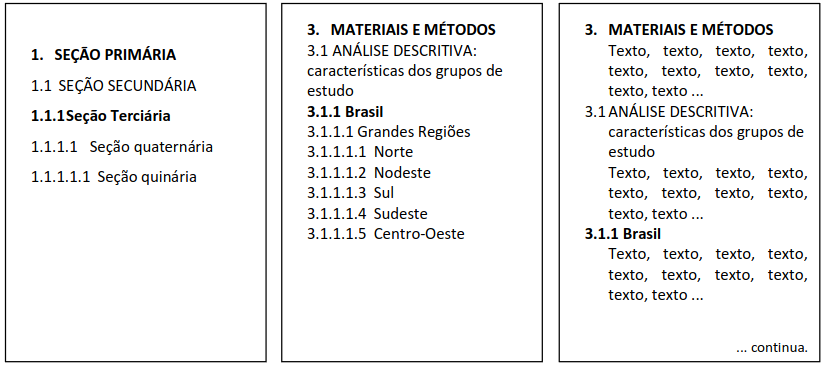
\includegraphics[width=0.75\textwidth,height=\textheight]{figuras/secao-subsecao.png}

}

\end{figure}
\end{frame}

\begin{frame}[fragile]{\texttt{markdown}\newline Sintaxe básica}
\protect\hypertarget{markdownsintaxe-buxe1sica-1}{}
Podemos definir seções e subseções com \texttt{\#}.

\colorbox{cabecalho}{\textcolor{titulo}{O caractere \texttt{\#} precisa estar na primeira coluna da linha.}}\newline
\colorbox{cabecalho}{\textcolor{titulo}{É necessário incluir um único espaço depois de \texttt{\#}.}}

\begin{longtable}[]{@{}lll@{}}
\toprule\noalign{}
código \texttt{markdown} & código \texttt{HTML} & código \LaTeX \\
\midrule\noalign{}
\endhead
\texttt{\#\ texto} &
\texttt{\textless{}h1\textgreater{}texto\textless{}/h1\textgreater{}} &
\texttt{\textbackslash{}section\{texto\}} \\
\texttt{\#\#\ texto} &
\texttt{\textless{}h2\textgreater{}texto\textless{}/h2\textgreater{}} &
\texttt{\textbackslash{}subsection\{texto\}} \\
\texttt{\#\#\#\ texto} &
\texttt{\textless{}h3\textgreater{}texto\textless{}/h3\textgreater{}} &
\texttt{\textbackslash{}subsubsection\{texto\}} \\
\texttt{\#\#\#\#\ texto} &
\texttt{\textless{}h4\textgreater{}texto\textless{}/h4\textgreater{}} &
\texttt{\textbackslash{}paragraph\{texto\}} \\
\texttt{\#\#\#\#\#\ texto} &
\texttt{\textless{}h5\textgreater{}texto\textless{}/h5\textgreater{}} &
\texttt{\textbackslash{}subparagraph\{texto\}} \\
\texttt{\#\#\#\#\#\#\ texto} &
\texttt{\textless{}h6\textgreater{}texto\textless{}/h6\textgreater{}}
& \\
\bottomrule\noalign{}
\end{longtable}
\end{frame}

\begin{frame}[fragile]{\texttt{markdown}\newline Sintaxe básica}
\protect\hypertarget{markdownsintaxe-buxe1sica-2}{}
\textbf{Parágrafos}

Para criar parágrafos, separa blocos de linhas com um (ou mais) linhas
em branco.

\begin{longtable}[]{@{}lll@{}}
\toprule\noalign{}
código \texttt{markdown} & código \texttt{HTML} & código \LaTeX \\
\midrule\noalign{}
\endhead
\texttt{Primeira\ linha.} &
\texttt{\textless{}p\textgreater{}Primeira\ linha.\textless{}/p\textgreater{}}
& \texttt{Primeira\ linha.} \\
&
\texttt{\textless{}p\textgreater{}Segunda\ linha.\textless{}/p\textgreater{}}
& \\
\texttt{Segunda\ linha.} & & \texttt{Segunda\ linha.} \\
\bottomrule\noalign{}
\end{longtable}

\textbf{Não inclua tabs ou espaços na primeira linha de parágrafos.}
\end{frame}

\begin{frame}[fragile]{\texttt{markdown}\newline Sintaxe básica}
\protect\hypertarget{markdownsintaxe-buxe1sica-3}{}
\textbf{Formatação de texto}

\scriptsize

\begin{longtable}[]{@{}
  >{\raggedright\arraybackslash}p{(\columnwidth - 8\tabcolsep) * \real{0.2727}}
  >{\raggedright\arraybackslash}p{(\columnwidth - 8\tabcolsep) * \real{0.1818}}
  >{\raggedright\arraybackslash}p{(\columnwidth - 8\tabcolsep) * \real{0.1818}}
  >{\raggedright\arraybackslash}p{(\columnwidth - 8\tabcolsep) * \real{0.1818}}
  >{\centering\arraybackslash}p{(\columnwidth - 8\tabcolsep) * \real{0.1818}}@{}}
\toprule\noalign{}
\begin{minipage}[b]{\linewidth}\raggedright
Descrição
\end{minipage} & \begin{minipage}[b]{\linewidth}\raggedright
código \texttt{markdown}
\end{minipage} & \begin{minipage}[b]{\linewidth}\raggedright
código \texttt{HTML}
\end{minipage} & \begin{minipage}[b]{\linewidth}\raggedright
código \LaTeX
\end{minipage} & \begin{minipage}[b]{\linewidth}\centering
Resultado
\end{minipage} \\
\midrule\noalign{}
\endhead
Itálico & \texttt{*Itálico*} &
\texttt{\textless{}em\textgreater{}Itálico\textless{}/em\textgreater{}}
& \texttt{\textbackslash{}textit\{Itálico\}} & \emph{Itálico} \\
Negrito & \texttt{**Negrito**} &
\texttt{\textless{}strong\textgreater{}Negrito\textless{}/strong\textgreater{}}
& \texttt{\textbackslash{}textbf\{Negrito\}} & \textbf{Negrito} \\
Tachado &
\texttt{\textasciitilde{}\textasciitilde{}Tachado\textasciitilde{}\textasciitilde{}}
& \texttt{\textless{}s\textgreater{}Tachado\textless{}/s\textgreater{}}
& & \st{Tachado} \\
Sobrescrito & \texttt{x\^{}2\^{}} &
\texttt{x\textless{}sup\textgreater{}2\textless{}/sup\textgreater{}} & &
x\textsuperscript{2} \\
Subscrito & \texttt{t\textasciitilde{}0\textasciitilde{}} &
\texttt{t\textless{}sub\textgreater{}0\textless{}/sub\textgreater{}} & &
t\textsubscript{0} \\
\bottomrule\noalign{}
\end{longtable}

\normalsize

Podemos ter um texto em negrito e em itálico:

\begin{Shaded}
\begin{Highlighting}[]
\NormalTok{***Negrito e Itálico***}
\end{Highlighting}
\end{Shaded}
\end{frame}

\begin{frame}[fragile]{\texttt{markdown}\newline Sintaxe básica}
\protect\hypertarget{markdownsintaxe-buxe1sica-4}{}
\textbf{Bloco de citação}

Na primeira linha do parágrafo, inclua \texttt{\textgreater{}}.

\textbf{Exemplo de código}

\begin{Shaded}
\begin{Highlighting}[]
\AttributeTok{\textgreater{} Isto é uma citação.}
\end{Highlighting}
\end{Shaded}

\textbf{Resultado}

\hfill\break

\begin{quote}
Isto é uma citação.
\end{quote}
\end{frame}

\begin{frame}[fragile]{\texttt{markdown}\newline Sintaxe básica}
\protect\hypertarget{markdownsintaxe-buxe1sica-5}{}
\textbf{Bloco de citação com múltiplos parágrafos}

Adicione \texttt{\textgreater{}} em cada parágrafo e nos espaços em
branco entre os parágrafos.

\textbf{Exemplo de código}

\begin{Shaded}
\begin{Highlighting}[]
\AttributeTok{\textgreater{} Primeira linha do bloco de citação.}
\AttributeTok{\textgreater{}}
\AttributeTok{\textgreater{} Segunda linha do bloco de citação.}
\end{Highlighting}
\end{Shaded}

\textbf{Resultado}

\hfill\break

\begin{quote}
Primeira linha do bloco de citação.

Segunda linha do bloco de citação.
\end{quote}
\end{frame}

\begin{frame}[fragile]{\texttt{markdown}\newline Sintaxe básica}
\protect\hypertarget{markdownsintaxe-buxe1sica-6}{}
\textbf{Bloco de citação} pode ter todos os outros elementos
\texttt{markdown}.

\textbf{Exemplo}

\begin{Shaded}
\begin{Highlighting}[]
\AttributeTok{\textgreater{} \#\#\# Um lindo bloco de citação}
\AttributeTok{\textgreater{} Primeiro parágrafo tem **negrito**.}
\AttributeTok{\textgreater{}}
\AttributeTok{\textgreater{} Segundo parágrafo tem *Itálico*.}
\AttributeTok{\textgreater{}}
\AttributeTok{\textgreater{} Terceiro Páragrafo tem ***Negrito e Itálico***.}
\end{Highlighting}
\end{Shaded}

\textbf{Resultado}

\begin{quote}
\hypertarget{um-lindo-bloco-de-citauxe7uxe3o}{%
\subsubsection{Um lindo bloco de
citação}\label{um-lindo-bloco-de-citauxe7uxe3o}}

Primeiro parágrafo tem \textbf{negrito}.

Segundo parágrafo tem \emph{Itálico}.

Terceiro Páragrafo tem \textbf{\emph{Negrito e Itálico}}.
\end{quote}
\end{frame}

\begin{frame}[fragile]{\texttt{markdown}\newline Sintaxe básica}
\protect\hypertarget{markdownsintaxe-buxe1sica-7}{}
\textbf{Listas ordenadas}

As listas ordenadas devem começar com o número \texttt{1} (ou
\texttt{i.}).

\small

\begin{longtable}[]{@{}
  >{\raggedright\arraybackslash}p{(\columnwidth - 4\tabcolsep) * \real{0.3333}}
  >{\raggedright\arraybackslash}p{(\columnwidth - 4\tabcolsep) * \real{0.3333}}
  >{\raggedright\arraybackslash}p{(\columnwidth - 4\tabcolsep) * \real{0.3333}}@{}}
\toprule\noalign{}
\begin{minipage}[b]{\linewidth}\raggedright
código \texttt{markdown}
\end{minipage} & \begin{minipage}[b]{\linewidth}\raggedright
código \texttt{HTML}
\end{minipage} & \begin{minipage}[b]{\linewidth}\raggedright
código \LaTeX
\end{minipage} \\
\midrule\noalign{}
\endhead
\texttt{1.\ Primeiro\ item} & \texttt{\textless{}ol\textgreater{}} &
\texttt{\textbackslash{}begin\{enumerate\}} \\
\texttt{8.\ Segundo\ item} &
\quad\texttt{\textless{}li\textgreater{}Primeiro\ item\textless{}/li\textgreater{}}
& \quad \texttt{\textbackslash{}item\ Primeiro\ item} \\
\texttt{1.\ Terceiro\ item} &
\quad\texttt{\textless{}li\textgreater{}Segundo\ item\textless{}/li\textgreater{}}
& \quad \texttt{\textbackslash{}item\ Segundo\ item} \\
&
\quad\texttt{\textless{}li\textgreater{}Terceiro\ item\textless{}/li\textgreater{}}
& \quad \texttt{\textbackslash{}item\ Terceiro\ item} \\
& \texttt{\textless{}/ol\textgreater{}} &
\texttt{\textbackslash{}end\{enumerate\}} \\
\bottomrule\noalign{}
\end{longtable}

\normalsize

\textbf{Resultado}

\begin{enumerate}
\tightlist
\item
  Primeiro item
\item
  Segundo item
\item
  Terceiro item
\end{enumerate}
\end{frame}

\begin{frame}[fragile]{\texttt{markdown}\newline Sintaxe básica}
\protect\hypertarget{markdownsintaxe-buxe1sica-8}{}
\textbf{Listas não ordenadas}

As listas não ordenadas começam com: \texttt{-}, \texttt{*} ou
\texttt{+}.

\small

\begin{longtable}[]{@{}
  >{\raggedright\arraybackslash}p{(\columnwidth - 4\tabcolsep) * \real{0.3333}}
  >{\raggedright\arraybackslash}p{(\columnwidth - 4\tabcolsep) * \real{0.3333}}
  >{\raggedright\arraybackslash}p{(\columnwidth - 4\tabcolsep) * \real{0.3333}}@{}}
\toprule\noalign{}
\begin{minipage}[b]{\linewidth}\raggedright
código \texttt{markdown}
\end{minipage} & \begin{minipage}[b]{\linewidth}\raggedright
código \texttt{HTML}
\end{minipage} & \begin{minipage}[b]{\linewidth}\raggedright
código \LaTeX
\end{minipage} \\
\midrule\noalign{}
\endhead
\texttt{+\ Primeiro\ item} & \texttt{\textless{}ul\textgreater{}} &
\texttt{\textbackslash{}begin\{itemize\}} \\
\texttt{+\ Segundo\ item} &
\quad\texttt{\textless{}li\textgreater{}Primeiro\ item\textless{}/li\textgreater{}}
& \quad \texttt{\textbackslash{}item\ Primeiro\ item} \\
\texttt{+\ Terceiro\ item} &
\quad\texttt{\textless{}li\textgreater{}Segundo\ item\textless{}/li\textgreater{}}
& \quad \texttt{\textbackslash{}item\ Segundo\ item} \\
&
\quad\texttt{\textless{}li\textgreater{}Terceiro\ item\textless{}/li\textgreater{}}
& \quad \texttt{\textbackslash{}item\ Terceiro\ item} \\
& \texttt{\textless{}/ul\textgreater{}} &
\texttt{\textbackslash{}end\{itemize\}} \\
\bottomrule\noalign{}
\end{longtable}

\normalsize

\textbf{Resultado}

\begin{itemize}
\tightlist
\item
  Primeiro item
\item
  Segundo item
\item
  Terceiro item
\end{itemize}
\end{frame}

\begin{frame}[fragile]{\texttt{markdown}\newline Sintaxe básica}
\protect\hypertarget{markdownsintaxe-buxe1sica-9}{}
\textbf{Listas aninhadas}

Indente as listas que estão dentro de outras listas com dois espaços.

\scriptsize

\begin{longtable}[]{@{}
  >{\raggedright\arraybackslash}p{(\columnwidth - 4\tabcolsep) * \real{0.3333}}
  >{\raggedright\arraybackslash}p{(\columnwidth - 4\tabcolsep) * \real{0.3333}}
  >{\raggedright\arraybackslash}p{(\columnwidth - 4\tabcolsep) * \real{0.3333}}@{}}
\toprule\noalign{}
\begin{minipage}[b]{\linewidth}\raggedright
código \texttt{markdown}
\end{minipage} & \begin{minipage}[b]{\linewidth}\raggedright
código \texttt{HTML}
\end{minipage} & \begin{minipage}[b]{\linewidth}\raggedright
código \LaTeX
\end{minipage} \\
\midrule\noalign{}
\endhead
\texttt{+\ Item\ 1} & \texttt{\textless{}ul\textgreater{}} &
\texttt{\textbackslash{}begin\{itemize\}} \\
\quad\texttt{+\ Item\ 1\ interno} &
\quad\texttt{\textless{}li\textgreater{}Item\ 1\textless{}/li\textgreater{}}
& \quad \texttt{\textbackslash{}item\ Item\ 1} \\
\quad\texttt{+\ Item\ 2\ interno} &
\quad\texttt{\textless{}ul\textgreater{}} &
\quad \texttt{\textbackslash{}begin\{itemize\}} \\
\texttt{+\ Item\ 2} &
\quad\quad\texttt{\textless{}li\textgreater{}Item\ 1\ interno\textless{}/li\textgreater{}}
& \quad\quad \texttt{\textbackslash{}item\ Item\ 1\ interno} \\
&
\quad\quad\texttt{\textless{}li\textgreater{}Item\ 2\ interno\textless{}/li\textgreater{}}
& \quad\quad \texttt{\textbackslash{}item\ Item\ 2\ interno} \\
& \quad\texttt{\textless{}/ul\textgreater{}} &
\quad \texttt{\textbackslash{}end\{itemize\}} \\
&
\quad\texttt{\textless{}li\textgreater{}Item\ 2\textless{}/li\textgreater{}}
& \quad \texttt{\textbackslash{}item\ Item\ 2} \\
& \texttt{\textless{}/ul\textgreater{}} &
\texttt{\textbackslash{}end\{itemize\}} \\
\bottomrule\noalign{}
\end{longtable}

\normalsize

\textbf{Resultado}

\begin{itemize}
\tightlist
\item
  Item 1

  \begin{itemize}
  \tightlist
  \item
    Item 1
  \item
    Item 2
  \end{itemize}
\item
  Item 2
\end{itemize}
\end{frame}

\begin{frame}[fragile]{\texttt{markdown}\newline Sintaxe básica}
\protect\hypertarget{markdownsintaxe-buxe1sica-10}{}
\textbf{Listas aninhadas}

Indente as listas que estão dentro de outras listas com dois espaços.

\scriptsize

\begin{longtable}[]{@{}
  >{\raggedright\arraybackslash}p{(\columnwidth - 4\tabcolsep) * \real{0.3333}}
  >{\raggedright\arraybackslash}p{(\columnwidth - 4\tabcolsep) * \real{0.3333}}
  >{\raggedright\arraybackslash}p{(\columnwidth - 4\tabcolsep) * \real{0.3333}}@{}}
\toprule\noalign{}
\begin{minipage}[b]{\linewidth}\raggedright
código \texttt{markdown}
\end{minipage} & \begin{minipage}[b]{\linewidth}\raggedright
código \texttt{HTML}
\end{minipage} & \begin{minipage}[b]{\linewidth}\raggedright
código \LaTeX
\end{minipage} \\
\midrule\noalign{}
\endhead
\texttt{+\ Item\ 1} & \texttt{\textless{}ul\textgreater{}} &
\texttt{\textbackslash{}begin\{itemize\}} \\
\quad\texttt{1.\ Item\ 1\ interno} &
\quad\texttt{\textless{}li\textgreater{}Item\ 1\textless{}/li\textgreater{}}
& \quad \texttt{\textbackslash{}item\ Item\ 1} \\
\quad\texttt{1.\ Item\ 2\ interno} &
\quad\texttt{\textless{}ol\textgreater{}} &
\quad \texttt{\textbackslash{}begin\{enumerate\}} \\
\texttt{+\ Item\ 2} &
\quad\quad\texttt{\textless{}li\textgreater{}Item\ 1\ interno\textless{}/li\textgreater{}}
& \quad\quad \texttt{\textbackslash{}item\ Item\ 1\ interno} \\
&
\quad\quad\texttt{\textless{}li\textgreater{}Item\ 2\ interno\textless{}/li\textgreater{}}
& \quad\quad \texttt{\textbackslash{}item\ Item\ 2\ interno} \\
& \quad\texttt{\textless{}/ol\textgreater{}} &
\quad \texttt{\textbackslash{}end\{enumerate\}} \\
&
\quad\texttt{\textless{}li\textgreater{}Item\ 2\textless{}/li\textgreater{}}
& \quad \texttt{\textbackslash{}item\ Item\ 2} \\
& \texttt{\textless{}/ul\textgreater{}} &
\texttt{\textbackslash{}end\{itemize\}} \\
\bottomrule\noalign{}
\end{longtable}

\normalsize

\textbf{Resultado}

\begin{itemize}
\tightlist
\item
  Item 1

  \begin{enumerate}
  \tightlist
  \item
    Item 1
  \item
    Item 2
  \end{enumerate}
\item
  Item 2
\end{itemize}
\end{frame}

\begin{frame}[fragile]{\texttt{markdown}\newline Sintaxe básica}
\protect\hypertarget{markdownsintaxe-buxe1sica-11}{}
\textbf{Código fonte (sem inclusão do resultado)}

Para inclusão de código \emph{inline} (dentro de uma frase):
\texttt{\textasciigrave{}print("olá\ mundo!")\textasciigrave{}}.

\textbf{Exemplo}

\begin{Shaded}
\begin{Highlighting}[]
\NormalTok{Um texto com código }\InformationTok{\textasciigrave{}print(1 + 2)\textasciigrave{}}\NormalTok{.}
\end{Highlighting}
\end{Shaded}

\textbf{Resultado}

Um texto com código \texttt{print(1\ +\ 2)}.
\end{frame}

\begin{frame}[fragile]
Para inclusão de código \emph{em bloco}, use
\texttt{\textasciigrave{}\textasciigrave{}\textasciigrave{}}.

\textbf{Exemplo}

Podemos substituir \texttt{r} por: \texttt{python}, \texttt{html},
\texttt{julia} entre outros.

\texttt{\textasciigrave{}\textasciigrave{}\textasciigrave{}r}\newline
\texttt{print("Olá\ mundo!")}\newline \texttt{print(1\ +\ 2)}\newline
\texttt{\textasciigrave{}\textasciigrave{}\textasciigrave{}}

\textbf{Resultado}

\begin{Shaded}
\begin{Highlighting}[]
\FunctionTok{print}\NormalTok{(}\StringTok{"Olá mundo"}\NormalTok{)}
\FunctionTok{print}\NormalTok{(}\DecValTok{1} \SpecialCharTok{+} \DecValTok{2}\NormalTok{)}
\end{Highlighting}
\end{Shaded}

Para ver a lista de linguagens compatíveis consulte:
\href{https://github.com/jgm/skylighting/tree/master/skylighting-core/xml}{linguagens
compatíveis com \texttt{markdown}}.
\end{frame}

\begin{frame}[fragile]{\texttt{markdown}\newline Sintaxe básica}
\protect\hypertarget{markdownsintaxe-buxe1sica-12}{}
\textbf{Tabelas}

\texttt{markdown} usa tabelas conhecidas como \texttt{pipe\ table} que
tem a seguinte sintaxe:

\begin{itemize}
\tightlist
\item
  As colunas são separadas por \texttt{\textbar{}}.
\item
  A primeira linha contém cabeçalho das colunas.
\item
  A segunda linha contém o alinhamento:

  \begin{itemize}
  \tightlist
  \item
    \texttt{-\/-\/-\/-\/-} (default) valores serão alinhados à esquerda
  \item
    \texttt{-\/-\/-\/-:} valores serão alinhados à direita
  \item
    \texttt{:-\/-\/-\/-} valores serão alinhados à esquerda
  \item
    \texttt{:-\/-\/-:} valores ficarão centralizados
  \end{itemize}
\item
  A partir da terceira linha, incluimos as informações
\item
  Incluímos a legenda da tabela depois de incluirmos todas as linhas
\end{itemize}
\end{frame}

\begin{frame}[fragile]
\destaque{As células de uma \textit{pipe table} \textbf{não} podem conter:} 
\begin{itemize}
    \item \destaque{parágrafos}
    \item \destaque{listas}
    \item \destaque{valor em múltiplas linhas}
\end{itemize}

Gerador de tabelas \texttt{markdown}:
\href{https://www.tablesgenerator.com/markdown_tables}{tablesgenerator.com/markdown\_tables}.
\end{frame}

\begin{frame}[fragile]
\textbf{Exemplo}

\scriptsize

\begin{Shaded}
\begin{Highlighting}[]
\NormalTok{| default | alinhamento à esquerda | alinhamento à direita | centralizado |}
\NormalTok{|{-}{-}{-}{-}{-}{-}{-}{-}{-}|:{-}{-}{-}{-}{-}|{-}{-}{-}{-}{-}{-}:|:{-}{-}{-}{-}{-}{-}:|}
\NormalTok{|12|12|12|12|}
\NormalTok{|123|123|123|123|}
\NormalTok{|1|1|1|1|}

\NormalTok{: Legenda da tabela.}
\end{Highlighting}
\end{Shaded}

\normalsize

\textbf{Resultado}

\begin{longtable}[]{@{}
  >{\raggedright\arraybackslash}p{(\columnwidth - 6\tabcolsep) * \real{0.3000}}
  >{\raggedright\arraybackslash}p{(\columnwidth - 6\tabcolsep) * \real{0.2000}}
  >{\raggedleft\arraybackslash}p{(\columnwidth - 6\tabcolsep) * \real{0.2333}}
  >{\centering\arraybackslash}p{(\columnwidth - 6\tabcolsep) * \real{0.2667}}@{}}
\caption{Legenda da tabela.}\tabularnewline
\toprule\noalign{}
\begin{minipage}[b]{\linewidth}\raggedright
default
\end{minipage} & \begin{minipage}[b]{\linewidth}\raggedright
alinhamento à esquerda
\end{minipage} & \begin{minipage}[b]{\linewidth}\raggedleft
alinhamento à direita
\end{minipage} & \begin{minipage}[b]{\linewidth}\centering
centralizado
\end{minipage} \\
\midrule\noalign{}
\endfirsthead
\toprule\noalign{}
\begin{minipage}[b]{\linewidth}\raggedright
default
\end{minipage} & \begin{minipage}[b]{\linewidth}\raggedright
alinhamento à esquerda
\end{minipage} & \begin{minipage}[b]{\linewidth}\raggedleft
alinhamento à direita
\end{minipage} & \begin{minipage}[b]{\linewidth}\centering
centralizado
\end{minipage} \\
\midrule\noalign{}
\endhead
12 & 12 & 12 & 12 \\
123 & 123 & 123 & 123 \\
1 & 1 & 1 & 1 \\
\bottomrule\noalign{}
\end{longtable}
\end{frame}

\begin{frame}[fragile]{\texttt{markdown}\newline Sintaxe básica}
\protect\hypertarget{markdownsintaxe-buxe1sica-13}{}
\textbf{Links e imagens}

A sintaxe básica para links é
\texttt{{[}texto\ do\ link{]}(endereço\ do\ link)}, onde:

\begin{itemize}
\tightlist
\item
  \texttt{texto\ do\ link} é um texto descritivo para o link
\item
  \texttt{endereço\ do\ link} é o endereço para redirecionamento
\end{itemize}

\textbf{Exemplo:}

\begin{Shaded}
\begin{Highlighting}[]
\CommentTok{[}\OtherTok{Google}\CommentTok{](https://www.google.com.br)}
\end{Highlighting}
\end{Shaded}

\textbf{Resultado:}

\href{https://www.google.com.br}{Google}

\regrafina

Se \textbf{\emph{\texttt{texto\ do\ link}}} é igual a
\textbf{\emph{\texttt{endereço\ do\ link}}}, você pode usar:

\begin{Shaded}
\begin{Highlighting}[]
\OtherTok{\textless{}https://www.google.com.br\textgreater{}}
\end{Highlighting}
\end{Shaded}
\end{frame}

\begin{frame}[fragile]{\texttt{markdown}\newline Sintaxe básica}
\protect\hypertarget{markdownsintaxe-buxe1sica-14}{}
\textbf{Links e imagens}

A sintaxe básica para links é
\texttt{!{[}texto\ da\ imagem{]}(endereço\ da\ imagem)}, onde:

\begin{itemize}
\tightlist
\item
  \texttt{texto\ da\ imagem} é um texto descritivo da imagem
\item
  \texttt{endereço\ da\ imagem} é \emph{filename} da imagem
\end{itemize}

\destaque{A imagem precisa estar dentro do mesmo diretório que o arquivo \texttt{.Rmd}.}

\textbf{Exemplo}

\begin{Shaded}
\begin{Highlighting}[]
\AlertTok{![Logo da linguagem R](figuras/r.png)}
\end{Highlighting}
\end{Shaded}
\end{frame}

\begin{frame}
\textbf{Resultado}

\begin{figure}

{\centering 
\includegraphics{figuras/r.png}

}

\caption{Logo da linguagem R}

\end{figure}
\end{frame}

\begin{frame}[fragile]{\texttt{markdown}\newline Sintaxe básica}
\protect\hypertarget{markdownsintaxe-buxe1sica-15}{}
\textbf{Exemplo}

\begin{itemize}
\tightlist
\item
  Vamos analisar um documento simples usando \texttt{markdown}.
\item
  Por hora, ignore as primeiras linhas delimitadas \texttt{-\/-\/-}.
\end{itemize}

\href{https://ufbabr-my.sharepoint.com/:u:/g/personal/gilberto_sassi_ufba_br/EVkS8aZN8rZDqXEJXXVFWzIBfkqMGhKClWZ5Mbmiv6vh4g?e=apQKvV}{Exemplo
com sintaxe}
\end{frame}

\begin{frame}[fragile]{\texttt{markdown}\newline Sintaxe básica}
\protect\hypertarget{markdownsintaxe-buxe1sica-16}{}
\textbf{Exercício}

\small

Use \href{https://loremipsum.io/}{loremipsum.io} para criar um texto
\texttt{html}.

Inclua:

\begin{itemize}
\tightlist
\item
  o texto precisa ter 6 parágrafos
\item
  uma citação de sua preferência
\item
  texto negrito, texto itálico, texto tachado, e texto tachado e negrito
\item
  inclua uma lista de itens que você gosta
\item
  inclua a seguinte tabela com as colunas centralizadas
\item
  inclua um link para o website do nosso curso
  \href{https://rmarkdown.simple.ink}{rmarkdown.simple.ink}
\item
  inclua o logo rmarkdown ao final do arquivo (o arquivo na pasta
  \texttt{figuras})
\end{itemize}

\begin{longtable}[]{@{}lr@{}}
\toprule\noalign{}
Cidade & População \\
\midrule\noalign{}
\endhead
São Paulo & 11.451.245 \\
Rio de Janeiro & 6.211.423 \\
Brasília & 2.817.068 \\
Fortaleza & 2.428.678 \\
Salvador & 2.418.005 \\
\bottomrule\noalign{}
\end{longtable}

\normalsize
\end{frame}

\hypertarget{equauxe7uxf5es-usando}{%
\section{\texorpdfstring{Equações usando
\LaTeX}{Equações usando }}\label{equauxe7uxf5es-usando}}

\begin{frame}[fragile]{Expressões matemáticas usando \LaTeX}
\protect\hypertarget{expressuxf5es-matemuxe1ticas-usando}{}
\texttt{rmarkdown} e \texttt{quarto} usam
\href{https://en.wikibooks.org/wiki/LaTeX}{\LaTeX}~para composição
tipográfica de equações matemáticas.

Existem dois tipos de inclusão de equações matemáticas:

\begin{itemize}
\tightlist
\item
  \emph{inline}: equação é parte de um parágrafo

  \begin{itemize}
  \tightlist
  \item
    usamos \texttt{\$} para equações em modo \emph{inline}
  \end{itemize}
\item
  \emph{display}: equação em um linha separada com texto centralizado

  \begin{itemize}
  \tightlist
  \item
    usamos \texttt{\$\$}para equações em modo \emph{display}
  \end{itemize}
\end{itemize}
\end{frame}

\begin{frame}[fragile]{Expressões matemáticas usando
\LaTeX\newline Equações em modo \emph{inline}}
\protect\hypertarget{expressuxf5es-matemuxe1ticas-usando-equauxe7uxf5es-em-modo-inline}{}
\textbf{Exemplo:}

\begin{Shaded}
\begin{Highlighting}[]
\NormalTok{A equação $e\^{}\{i\textbackslash{}pi\} + 1=0$ foi proposta por Euler.}
\end{Highlighting}
\end{Shaded}

\textbf{Resultado:}

A equação \(e^{i\pi} + 1=0\) foi proposta por Euler.
\end{frame}

\begin{frame}[fragile]{Expressões matemáticas usando
\LaTeX\newline Equações em modo \emph{display}}
\protect\hypertarget{expressuxf5es-matemuxe1ticas-usando-equauxe7uxf5es-em-modo-display}{}
\textbf{Exemplo:}

\begin{Shaded}
\begin{Highlighting}[]
\AnnotationTok{A seguinte equação foi proposta por Euler:}
\NormalTok{$$}
\NormalTok{e\^{}\{i\textbackslash{}pi\} + 1=0}
\NormalTok{$$}
\end{Highlighting}
\end{Shaded}

\textbf{Resultado:}

A seguinte equação foi proposta por Euler: \[
e^{i\pi} + 1=0
\]
\end{frame}

\begin{frame}[fragile]{Expressões matemáticas usando
\LaTeX\newline Símbolos e funções importantes}
\protect\hypertarget{expressuxf5es-matemuxe1ticas-usando-suxedmbolos-e-funuxe7uxf5es-importantes}{}
\scriptsize

\begin{longtable}[]{@{}llr@{}}
\toprule\noalign{}
Descrição & Código \LaTeX & Resultado \\
\midrule\noalign{}
\endhead
Letra alpha & \texttt{\textbackslash{}alpha} & \(\alpha\) \\
Letra epsilon & \texttt{\textbackslash{}epsilon} & \(\epsilon\) \\
União de conjuntos & \texttt{\textbackslash{}cup} & \(\cup\) \\
Intersecção de conjuntos & \texttt{\textbackslash{}cap} & \(\cap\) \\
Menor (desigualdade) & \texttt{\textless{}} & \(<\) \\
Espaço simples & \texttt{b\textbackslash{}\ a} & \(b\ a\) \\
Espaço duplo & \texttt{b\textbackslash{}quad\ a} & \(b\quad a\) \\
Espaço triplo & \texttt{b\textbackslash{}qquad\ a} & \(b\qquad a\) \\
Maior (desigualdade) & \texttt{\textgreater{}} & \(>\) \\
Infinito & \texttt{\textbackslash{}infty} & \(\infty\) \\
Logaritmo & \texttt{\textbackslash{}log} & \(\log\) \\
Multiplicação & \texttt{\textbackslash{}cdot} & \(\cdot\) \\
Contém & \texttt{\textbackslash{}subset} & \(\subset\) \\
Contido & \texttt{\textbackslash{}supset} & \(\supset\) \\
Integral & \texttt{\textbackslash{}int} & \(\int\) \\
Somatório & \texttt{\textbackslash{}sum} & \(\sum\) \\
Produtório & \texttt{\textbackslash{}prod} & \(\prod\) \\
Limite & \texttt{\textbackslash{}lim} & \(\lim\) \\
\bottomrule\noalign{}
\end{longtable}

\normalsize

\href{https://en.wikibooks.org/wiki/LaTeX/Mathematics\#Symbols}{Lista
exaustiva de símbolos e funções}.

\href{https://detexify.kirelabs.org/classify.html}{Detexfy - aplicativo
para descobrir símbolos matemáticos}.
\end{frame}

\begin{frame}[fragile]{Expressões matemáticas usando
\LaTeX\newline Sobrescrito, subscrito e fração}
\protect\hypertarget{expressuxf5es-matemuxe1ticas-usando-sobrescrito-subscrito-e-frauxe7uxe3o}{}
\textbf{Sobrescrito e subscrito}

Muito comum em expressões matemáticas envolvendo expoentes, índices, e
em alguns proponentes especiais.

\begin{itemize}
\tightlist
\item
  Sobrescrito e limite superior em \(\int\), \(\prod\), \(\sum\),
  \(\cap\) e \(\cup\): \texttt{\^{}}
\item
  Subscrito e limite inferior em em \(\int\), \(\prod\), \(\sum\),
  \(\cap\) e \(\cup\): \texttt{\_}
\end{itemize}

Se o sobrescrito e subscrito tiver mais de um caracter, envolva a
expressão em chaves \texttt{\{\}}.

\regrafina

\textbf{Fração}

\begin{longtable}[]{@{}ll@{}}
\toprule\noalign{}
Código \LaTeX & Resultado \\
\midrule\noalign{}
\endhead
\texttt{\textbackslash{}frac\{a\}\{b\}} & \(\frac{a}{b}\) \\
\bottomrule\noalign{}
\end{longtable}
\end{frame}

\begin{frame}[fragile]{Expressões matemáticas usando
\LaTeX\newline Sobrescrito e subscrito}
\protect\hypertarget{expressuxf5es-matemuxe1ticas-usando-sobrescrito-e-subscrito}{}
\begin{longtable}[]{@{}
  >{\raggedright\arraybackslash}p{(\columnwidth - 2\tabcolsep) * \real{0.4545}}
  >{\raggedleft\arraybackslash}p{(\columnwidth - 2\tabcolsep) * \real{0.5455}}@{}}
\toprule\noalign{}
\begin{minipage}[b]{\linewidth}\raggedright
Código \LaTeX
\end{minipage} & \begin{minipage}[b]{\linewidth}\raggedleft
Resultado
\end{minipage} \\
\midrule\noalign{}
\endhead
\texttt{a\^{}\{n\_j\}} & \(a^{n_j}\) \\
\texttt{a\_\{n\^{}i\}} & \(a_{n^i}\) \\
\texttt{\textbackslash{}int\_\{-\textbackslash{}infty\}\^{}\{\textbackslash{}infty\}\ \textbackslash{}frac\{1\}\{1\ +\ x\^{}2\}\ dx}
& \(\int_{-\infty}^{\infty} \frac{1}{1 + x^2} dx\) \\
\texttt{\textbackslash{}sum\_\{i=1\}\^{}\{\textbackslash{}infty\}\ \textbackslash{}frac\{1\}\{i\^{}2\}}
& \(\sum_{i=1}^{\infty} \frac{1}{i^2}\) \\
\texttt{\textbackslash{}prod\_\{i=1\}\^{}n\ i} & \(\prod_{i=1}^n i\) \\
\texttt{\textbackslash{}cup\_\{i=1\}\^{}\{n+12\}\ A\_i} &
\(\cup_{i=1}^{n+12} A_i\) \\
\texttt{\textbackslash{}cap\_\{i=-\textbackslash{}infty\}\^{}0\ B\_i} &
\(\cap_{i=-\infty}^0 B_i\) \\
\bottomrule\noalign{}
\end{longtable}
\end{frame}

\begin{frame}[fragile]{Expressões matemáticas usando
\LaTeX\newline Parênteses, colchetes e chaves}
\protect\hypertarget{expressuxf5es-matemuxe1ticas-usando-paruxeanteses-colchetes-e-chaves}{}
\normalsize

\begin{longtable}[]{@{}llr@{}}
\toprule\noalign{}
Descrição & Código \LaTeX & Resultado \\
\midrule\noalign{}
\endhead
Parênteses & \texttt{(x\ +\ y)} & \((x+y)\) \\
Colchetes & \texttt{{[}x\ +\ y{]}} & \([x+y]\) \\
Chaves & \texttt{\textbackslash{}\{x\ +\ y\textbackslash{}\}} &
\(\{x+y\}\) \\
Produto interno &
\texttt{\textbackslash{}langle\ x,\ y\ \textbackslash{}rangle} &
\(\langle x, y \rangle\) \\
Valor absoluto & \texttt{\textbar{}x\ +\ y\textbar{}} & \(|x + y|\) \\
Norma &
\texttt{\textbackslash{}\textbar{}x\ +\ y\textbackslash{}\textbar{}} &
\(\|x+y\|\) \\
Arrendonda para baixo &
\texttt{\textbackslash{}lfloor\ x\ +\ y\ \textbackslash{}rfloor} &
\(\lfloor x + y \rfloor\) \\
Arrendonda para cima &
\texttt{\textbackslash{}lceil\ x\ +\ y\ \textbackslash{}rceil} &
\(\lceil x + y \rceil\) \\
\bottomrule\noalign{}
\end{longtable}
\end{frame}

\begin{frame}[fragile]
Para aumentar o tamanho de parênteses, colchetes e outros:
\texttt{\textbackslash{}big}, \texttt{\textbackslash{}Big},
\texttt{\textbackslash{}bigg}, e \texttt{\textbackslash{}Bigg}.

Para aumentar o tamanho de parênteses, colchetes e outros:
\texttt{\textbackslash{}left} e \texttt{\textbackslash{}right} (na mesma
linha).

Para detalhes sobre ajuste no tamanho de parênteses, colchetes e outros,
consulte
\href{https://www.overleaf.com/learn/latex/Brackets_and_Parentheses}{parênteses,
colchetes e outros}.

\regrafina

Use \texttt{split} para quebrar uma equação em várias linhas, e use
\texttt{\&} para alinhamento.
\end{frame}

\begin{frame}[fragile]{Expressões matemáticas usando
\LaTeX\newline Parênteses, colchetes e chaves}
\protect\hypertarget{expressuxf5es-matemuxe1ticas-usando-paruxeanteses-colchetes-e-chaves-1}{}
\textbf{Exemplo}

\begin{Shaded}
\begin{Highlighting}[]
\SpecialStringTok{$$}
\KeywordTok{\textbackslash{}begin}\NormalTok{\{}\ExtensionTok{split}\NormalTok{\}}
\SpecialStringTok{a \&= }\SpecialCharTok{\textbackslash{}sum}\SpecialStringTok{\_\{i={-}}\SpecialCharTok{\textbackslash{}infty}\SpecialStringTok{\}\^{}\{}\SpecialCharTok{\textbackslash{}infty}\SpecialStringTok{\} }\SpecialCharTok{\textbackslash{}left\textbackslash{}\{}\SpecialStringTok{ a\_i + b\_i }\SpecialCharTok{\textbackslash{}right}\SpecialStringTok{.}\SpecialCharTok{\textbackslash{}\textbackslash{}}
\SpecialStringTok{\&= }\SpecialCharTok{\textbackslash{}left}\SpecialStringTok{. c\_i + }\SpecialCharTok{\textbackslash{}int}\SpecialStringTok{\_a\^{}b x }\SpecialCharTok{\textbackslash{}cdot}\SpecialStringTok{ i dx }\SpecialCharTok{\textbackslash{}right\textbackslash{}\}}
\KeywordTok{\textbackslash{}end}\NormalTok{\{}\ExtensionTok{split}\NormalTok{\}}
\SpecialStringTok{$$}
\end{Highlighting}
\end{Shaded}

\textbf{Resultado}

\[
\begin{split}
a &=  \sum_{i=-\infty}^{\infty} \left\{ a_i + b_i \right.\\
&= \left. c_i + \int_a^b x \cdot i\ dx \right\}
\end{split}
\]
\end{frame}

\begin{frame}{Expressões matemáticas usando \LaTeX\newline Exercício}
\protect\hypertarget{expressuxf5es-matemuxe1ticas-usando-exercuxedcio}{}
Use a plataforma \href{http://www.texrendr.com/}{www.texrendr.com} para
codificar em \LaTeX~as seguintes equações matemáticas:

\begin{itemize}
\tightlist
\item
  \(\sum_{i=0}^\infty \frac{1}{2^i} = 2\)
\item
  \(\int_{-\infty}^\infty \exp\left( -\frac{x^2}{2} \right)dx = \sqrt{2\pi}\)
\item
  \(\prod_{i=1}^n \frac{1}{2} = \frac{1}{2^n}\)
\item
  \(\lfloor 1,2 \rfloor = 1\)
\item
  \(\lceil 1,2 \rceil = 2\)
\item
  \(\|(1, 2)\|^2 = 5\)
\item
  \[\begin{split}\sum_{i=1}^{n} \alpha^i &= 1 + \alpha + \cdots + \alpha^n \\ &= \frac{1-\alpha^{n+1}}{1-\alpha} \end{split}\]
\end{itemize}
\end{frame}

\hypertarget{pacote-rmarkdown}{%
\section{\texorpdfstring{Pacote
\texttt{rmarkdown}}{Pacote rmarkdown}}\label{pacote-rmarkdown}}

\begin{frame}[fragile]{\texttt{rmarkdown}}
\protect\hypertarget{rmarkdown}{}
Documentos com extensão \texttt{.Rmd} ou \texttt{.rmd} permitem
combinar:

\begin{itemize}
\tightlist
\item
  código fonte (\texttt{code} tag in \texttt{html} e \texttt{verbatim}
  em \LaTeX)
\item
  resutaldo de computações
\item
  texto simples em prosa
\end{itemize}

Documentos com extensão \texttt{.Rmd} ou \texttt{.rmd} são renderizados
(processados) pelo pacote \texttt{rmarkdown}.

Gerador de texto aleatório para este curso:
\href{https://loremipsum.io/}{loremipsum.io}.

Cheatsheet do pacote \texttt{rmarkdown}:
\href{https://posit.co/wp-content/uploads/2022/10/rmarkdown-1.pdf}{cheatsheet
do pacote \texttt{rmarkdown}}.

\regrafina

\texttt{rmakdown} envia o documento \texttt{.Rmd} para o pacote
\texttt{knitr} que converte o documento para \texttt{markdown}, e em
seguida \texttt{pandoc} converte este arquivo \texttt{.md} para formato
adequado.

\begin{figure}

{\centering 
\includegraphics[width=0.5\textwidth,height=\textheight]{figuras/rmarkdown-flow.png}

}

\end{figure}
\end{frame}

\begin{frame}[fragile]{\texttt{rmarkdown}\newline RStudio}
\protect\hypertarget{rmarkdownrstudio}{}
\begin{enumerate}
\tightlist
\item
  Para criar um arquivo \texttt{.Rmd} no IDE
  \texttt{Rstudio}:\newline \texttt{file\ \textgreater{}\ New\ File\ \textgreater{}\ R\ Markdown}.
\item
  Em seguida, escolha a opção adequada para o seu texto, incluindo:

  \begin{enumerate}
  [a.]
  \tightlist
  \item
    \emph{document} (documentos em prosa).
  \item
    \emph{presentation} (apresentação).
  \item
    \emph{template} (documentos usando \emph{templates}).
  \end{enumerate}
\end{enumerate}
\end{frame}

\begin{frame}[fragile]{\texttt{rmarkdown}\newline Estrutura básica de
documentos \texttt{.Rmd}}
\protect\hypertarget{rmarkdownestrutura-buxe1sica-de-documentos-.rmd}{}
\tiny

\begin{Shaded}
\begin{Highlighting}[]
\NormalTok{{-}{-}{-}}
\NormalTok{title: "Um belo título para o documento"}
\NormalTok{date: 01{-}12{-}2023}
\NormalTok{output: html\_document}
\NormalTok{{-}{-}{-}}
\end{Highlighting}
\end{Shaded}

\texttt{\textasciigrave{}\textasciigrave{}\textasciigrave{}\{r\}}

\begin{Shaded}
\begin{Highlighting}[]
\NormalTok{\#| label: setup}
\NormalTok{\#| include: false}
\NormalTok{\#| echo: false}

\NormalTok{library(tidyverse)}
\end{Highlighting}
\end{Shaded}

\texttt{\textasciigrave{}\textasciigrave{}\textasciigrave{}}

\begin{Shaded}
\begin{Highlighting}[]
\NormalTok{\# Uma seção}

\NormalTok{Eu tenho 5 irmões.}

\NormalTok{Gráfico simples usando o pacote \textasciigrave{}ggplot2\textasciigrave{} do *framework* \textasciigrave{}tidyverse\textasciigrave{}.}
\end{Highlighting}
\end{Shaded}

\texttt{\textasciigrave{}\textasciigrave{}\textasciigrave{}\{r\}}

\begin{Shaded}
\begin{Highlighting}[]
\NormalTok{\#| echo: false}

\NormalTok{mtcars |\textgreater{}}
\NormalTok{  ggplot(aes(x = cyl)) +}
\NormalTok{  geom\_bar()}
\end{Highlighting}
\end{Shaded}

\texttt{\textasciigrave{}\textasciigrave{}\textasciigrave{}}

\begin{Shaded}
\begin{Highlighting}[]
\NormalTok{\#\# Uma subseção}

\NormalTok{Algum texto sobre alguma coisa muito importante.}
\end{Highlighting}
\end{Shaded}

\normalsize
\end{frame}

\begin{frame}[fragile]{\texttt{rmarkdown}\newline YAML}
\protect\hypertarget{rmarkdownyaml}{}
\small

\begin{itemize}
\tightlist
\item
  Criada em 2001.
\item
  YAML (Yet Another Markup Language) é uma linguagem desenvolvida para
  armazenar dados.
\item
  Fácil de ler e escrever.
\item
  YAML é delimitada por \texttt{-\/-\/-} e sempre está nas primeiras
  linhas do documento \texttt{.Rmd}.
\item
  YAML contrala a formatação do documento \texttt{.Rmd}.
\item
  YAML usa dupla \emph{chave valor}: \texttt{chave:\ valor}:

  \begin{itemize}
  \tightlist
  \item
    \texttt{valor} não pode ter espaço em branco. Se \texttt{valor}
    tiver espaço em branco, use aspas or \texttt{\textbar{}}.
  \item
    \texttt{chave}: nome do campo
  \end{itemize}
\end{itemize}

\begin{Shaded}
\begin{Highlighting}[]
\FunctionTok{title}\KeywordTok{:}\AttributeTok{ }\StringTok{"Um título que faz sentido"}
\end{Highlighting}
\end{Shaded}

ou

\begin{Shaded}
\begin{Highlighting}[]
\FunctionTok{title}\KeywordTok{: }\CharTok{|}
\NormalTok{  Um título que faz sentido}
\end{Highlighting}
\end{Shaded}

\normalsize
\end{frame}

\begin{frame}[fragile]
\texttt{valor} pode ter subcampos, e usamos indentação para neste
subcampo

\begin{Shaded}
\begin{Highlighting}[]
\FunctionTok{output}\KeywordTok{:}
\AttributeTok{  }\FunctionTok{html\_document}\KeywordTok{:}
\AttributeTok{    }\FunctionTok{highlight}\KeywordTok{:}\AttributeTok{ }\StringTok{"haddock"}
\AttributeTok{    }\FunctionTok{includes}\KeywordTok{:}
\AttributeTok{      }\FunctionTok{in\_header}\KeywordTok{:}\AttributeTok{ header.html}
\AttributeTok{      }\FunctionTok{before\_body}\KeywordTok{:}\AttributeTok{ before\_body.html        }
\end{Highlighting}
\end{Shaded}

\regrafina

Podemos usar código \texttt{R}, prefixando o campo com \texttt{!r}.

\begin{Shaded}
\begin{Highlighting}[]
\FunctionTok{date}\KeywordTok{:}\AttributeTok{ !r lubridate::today()}
\end{Highlighting}
\end{Shaded}

\regrafina

Campos comuns em YAML: \texttt{title}, \texttt{date} e \texttt{output}.
\end{frame}

\begin{frame}[fragile]{\texttt{rmarkdown}\newline YAML}
\protect\hypertarget{rmarkdownyaml-1}{}
\textbf{Citações e bibliografia}

\begin{itemize}
\tightlist
\item
  \texttt{rmarkdown} usa \href{https://tug.org/bibtex/}{\texttt{bibtex}}
  para incluir referências e citações.
\item
  \textbf{Google Scholar} e maioria das revistas científicas incluem
  citações \texttt{bibtex}.
\item
  Para espeficar um formato de bibliografia, use CSL (\emph{Citation
  Style Language}).
\end{itemize}

\begin{Shaded}
\begin{Highlighting}[]
\FunctionTok{bibliography}\KeywordTok{:}\AttributeTok{ refs.bib}
\FunctionTok{csl}\KeywordTok{:}\AttributeTok{ apa.csl}
\end{Highlighting}
\end{Shaded}
\end{frame}

\begin{frame}[fragile]
No texto, use \texttt{@} + identificador da referência no arquivo
\texttt{.bib}.

\begin{itemize}
\tightlist
\item
  Citação direta no texto: \texttt{@wickham2023r}.
\item
  Citação entre parenteses: \texttt{{[}@wickham2023r{]}}.
\item
  Cite apenas o ano entre parenteses: \texttt{{[}-@wickham2023r{]}}
\item
  Citação entre parenteses com comentário:
  \texttt{{[}veja\ @wickham2023r\ para\ mais\ detalhes{]}}.
\item
  Separe múltiplas citações com \texttt{;}:
  \texttt{{[}@wickham2023r;\ @wickham2019advanced;\ @xie2016bookdown{]}}
\end{itemize}
\end{frame}

\begin{frame}[fragile]{\texttt{rmarkdown}\newline YAML}
\protect\hypertarget{rmarkdownyaml-2}{}
\textbf{Parâmetros}

\begin{itemize}
\tightlist
\item
  Valores que passamos para os documentos.
\item
  Útil para produzir documentos em série, onde apenas alguns valores são
  modificados.
\item
  Valores ficam disponível na lista \texttt{params}.
\end{itemize}

\begin{Shaded}
\begin{Highlighting}[]
\FunctionTok{params}\KeywordTok{:}
\AttributeTok{  }\FunctionTok{nome}\KeywordTok{:}\AttributeTok{ }\StringTok{"Gilberto Pereira Sassi"}
\AttributeTok{  }\FunctionTok{idade}\KeywordTok{:}\AttributeTok{ }\DecValTok{22}
\end{Highlighting}
\end{Shaded}

\regrafina

No texto, use
\texttt{\textasciigrave{}r\ \ params\$nome\textasciigrave{}} e
\texttt{\textasciigrave{}r\ \ params\$idade\textasciigrave{}}.

Geralmente \texttt{params} é usado junto com a função \texttt{render} do
pacote \texttt{rmarkdown}.
\end{frame}

\begin{frame}[fragile]{\texttt{rmakrdown}\newline YAML}
\protect\hypertarget{rmakrdownyaml}{}
\textbf{Exemplo}

\scriptsize

\begin{Shaded}
\begin{Highlighting}[]
\NormalTok{{-}{-}{-}}
\NormalTok{title: "Seu título vem aqui"}
\NormalTok{date: 31/12/2023}
\NormalTok{output: html\_document}
\NormalTok{params:}
\NormalTok{  nome: "Nome da pessoa"}
\NormalTok{  vinculo: professor}
\NormalTok{{-}{-}{-}}

\NormalTok{\# Primeira seção}
\end{Highlighting}
\end{Shaded}

\texttt{Texto\ da\ primeira\ seção\ com\ o\ nome}
\texttt{\textasciigrave{}r\ \ params\$nome\textasciigrave{}}
\texttt{e\ Vínculo}
\texttt{\textasciigrave{}r\ \ params\$vinculo\textasciigrave{}}
\texttt{.}

\regrafina

Para produzir documento, use o seguinte código \texttt{R}

\begin{Shaded}
\begin{Highlighting}[]
\FunctionTok{render}\NormalTok{(}
  \StringTok{"filename.Rmd"}\NormalTok{,}
  \AttributeTok{render\_options =} \FunctionTok{list}\NormalTok{(}
    \AttributeTok{params =} \FunctionTok{list}\NormalTok{(}\AttributeTok{nome =} \StringTok{"Um nome"}\NormalTok{, }\AttributeTok{data =} \StringTok{"01/01/1900"}\NormalTok{)}
\NormalTok{  )}
\NormalTok{)}
\end{Highlighting}
\end{Shaded}

\normalsize
\end{frame}

\hypertarget{rmarkdown-ioslides_presentation}{%
\section{\texorpdfstring{\texttt{rmarkdown}\newline\newline~\texttt{ioslides\_presentation}}{rmarkdown~ioslides\_presentation}}\label{rmarkdown-ioslides_presentation}}

\begin{frame}[fragile]{\texttt{rmarkdown}\newline \texttt{ioslides\_presentation}}
\protect\hypertarget{rmarkdownioslides_presentation}{}
Apresentação em formato \texttt{.html}.

Para criar, especifique \texttt{output:\ ioslides\_presentation} no
cabeçalho YAML.

\begin{Shaded}
\begin{Highlighting}[]
\PreprocessorTok{{-}{-}{-}}
\FunctionTok{title}\KeywordTok{:}\AttributeTok{ }\StringTok{"Um lindo slide"}
\FunctionTok{author}\KeywordTok{:}\AttributeTok{ }\StringTok{"Fulano de Tal"}
\FunctionTok{date}\KeywordTok{:}\AttributeTok{ 01/01/1900}
\FunctionTok{output}\KeywordTok{:}\AttributeTok{ ioslides\_presentation}
\PreprocessorTok{{-}{-}{-}}
\end{Highlighting}
\end{Shaded}

\colorbox{cabecalho}{\textcolor{titulo}{Neste caso, você pode usar código \texttt{html} no texto.}}
\end{frame}

\begin{frame}[fragile]{\texttt{rmarkdown}\newline \texttt{ioslides\_presentation}}
\protect\hypertarget{rmarkdownioslides_presentation-1}{}
\small

Para adicionar um novo slide use \texttt{\#\#}:

\begin{Shaded}
\begin{Highlighting}[]
\FunctionTok{\#\# Um novo slide}

\NormalTok{Conteúdo do slide}
\end{Highlighting}
\end{Shaded}

Você pode adicionar um subtítulo do slide com \texttt{\textbar{}}:

\begin{Shaded}
\begin{Highlighting}[]
\FunctionTok{\#\# Título do slide | Subtítulo do slide}

\NormalTok{Conteúdo do slide}
\end{Highlighting}
\end{Shaded}

Se o slide estiver muito grande, você pode usar \texttt{-\/-\/-} para
quebrar o conteúdo:

\begin{Shaded}
\begin{Highlighting}[]
\FunctionTok{\#\# Título do slide | Subtítulo do slide}

\NormalTok{Conteúdo do slide}

\NormalTok{{-}{-}{-}}

\NormalTok{Essa parte vai para um novo slide}
\end{Highlighting}
\end{Shaded}

\normalsize
\end{frame}

\begin{frame}[fragile]{\texttt{rmarkdown}\newline \texttt{ioslides\_presentation}}
\protect\hypertarget{rmarkdownioslides_presentation-2}{}
O \texttt{ioslides} tem os seguintes modos de exibição:

\begin{itemize}
\tightlist
\item
  \texttt{f}: modo tela cheia
\item
  \texttt{w}: modo tela ampla
\item
  \texttt{o}: modo \emph{overview}
\item
  \texttt{h}: modo de destaque do código
\item
  \texttt{p}: modo de apresentação para o palestrante
\item
  \texttt{esc}: volta ao modo normal de apresentação
\end{itemize}
\end{frame}

\begin{frame}[fragile]{\texttt{rmarkdown}\newline \texttt{ioslides\_presentation}}
\protect\hypertarget{rmarkdownioslides_presentation-3}{}
Algumas configurações disponíveis no cabeçalho YAML:

\begin{itemize}
\tightlist
\item
  \texttt{incremental}: itens das listas são apresentadas um por um

  \begin{itemize}
  \tightlist
  \item
    Campo booleano (\texttt{true} - os itens das listas são apresentados
    um por um )
  \item
    Valor \texttt{default}: \texttt{false}
  \end{itemize}
\item
  \texttt{widescreen}: apresentação em modo de tela ampla

  \begin{itemize}
  \tightlist
  \item
    Campo booleano (\texttt{true} - a apresentação fica em tela ampla)
  \item
    Valor \texttt{default}: apresentação em modo de tela normal
  \end{itemize}
\item
  \texttt{smaller}: tamanho da fonte menor

  \begin{itemize}
  \tightlist
  \item
    Campo booleano: (\texttt{true} - tamanho da fonte fica um pouco
    menor)
  \item
    Valor \texttt{default}: tamanho normal (12pt)
  \end{itemize}
\item
  \texttt{transition}: velocidade de transição entre os slides

  \begin{itemize}
  \tightlist
  \item
    Valores possíveis: \texttt{default}, \texttt{slower},
    \texttt{faster}, ou número real que indica os segundos gastos na
    transição de slides:
  \item
    Valor \texttt{deafult}: \texttt{default}
  \end{itemize}
\item
  \texttt{logo}: adiciona a logo ao slide

  \begin{itemize}
  \tightlist
  \item
    Nome do arquivo. Por exemplo, \texttt{logo.png}
  \end{itemize}
\end{itemize}
\end{frame}

\begin{frame}[fragile]
Podemos incluir código \texttt{.html} para customização adicional da
apresentação com \texttt{includes}:

\begin{itemize}
\tightlist
\item
  \texttt{in\_header}: inclusão de código entre
  \texttt{\textless{}header\textgreater{}} e
  \texttt{\textless{}/header\textgreater{}}
\item
  \texttt{before\_body}: inclusão de código imediatamente depois
  \texttt{\textless{}body\textgreater{}}
\item
  \texttt{after\_body}: inclusão de código imediatamente antes de
  \texttt{\textless{}/body\textgreater{}}
\end{itemize}

\begin{Shaded}
\begin{Highlighting}[]
\FunctionTok{output}\KeywordTok{:}
\AttributeTok{  }\FunctionTok{pdf\_document}\KeywordTok{:}
\AttributeTok{    }\FunctionTok{includes}\KeywordTok{:}
\AttributeTok{      }\FunctionTok{in\_header}\KeywordTok{:}\AttributeTok{ in\_header.html}
\AttributeTok{      }\FunctionTok{before\_body}\KeywordTok{:}\AttributeTok{ before\_body.html}
\AttributeTok{      }\FunctionTok{after\_body}\KeywordTok{:}\AttributeTok{ after\_body.html}
\end{Highlighting}
\end{Shaded}
\end{frame}

\begin{frame}[fragile]{\texttt{rmarkdown}\newline \texttt{ioslides\_presentation}}
\protect\hypertarget{rmarkdownioslides_presentation-4}{}
Podemos fazer algumas configuraçãoes específicas para um slide.

\regrafina

Implementação da opção \texttt{incremental:\ true} para um único slide.

\begin{Shaded}
\begin{Highlighting}[]
\FunctionTok{\#\# Título do slide \{.build\}}
\end{Highlighting}
\end{Shaded}

\regrafina

Implementação da opção \texttt{smaller:\ true} para um único slide.

\begin{Shaded}
\begin{Highlighting}[]
\FunctionTok{\#\# Título do slide \{.build .smaller\}}
\end{Highlighting}
\end{Shaded}
\end{frame}

\begin{frame}[fragile]{\texttt{rmarkdown}\newline \texttt{ioslides\_presentation}}
\protect\hypertarget{rmarkdownioslides_presentation-5}{}
Para destacar um parte do código dentro de um \emph{chunk} usamos
\texttt{\#\#\ \textless{}b\textgreater{}} e
\texttt{\#\#\ \textless{}/b\textgreater{}}.

\regrafina

\textbf{Exemplo:}

\small

\texttt{\textasciigrave{}\textasciigrave{}\textasciigrave{}\{r\}}

\begin{Shaded}
\begin{Highlighting}[]
\NormalTok{library(tidyverse)}

\NormalTok{\#\# \textless{}b\textgreater{}}
\NormalTok{ggplot(airquality, aes(Ozone)) + geom\_histogram(bins = 8)}
\NormalTok{\#\# \textless{}/b\textgreater{}}

\NormalTok{summarise(}
\NormalTok{  media\_ozone = mean(Ozone), dp\_ozone = sd(Ozone),}
\NormalTok{  q1 = quantile(Ozone), mediana = median(Ozone),}
\NormalTok{  q3 = quantile(Ozone), cv\_ozone = dp\_ozone / media\_ozone}
\NormalTok{)}
\end{Highlighting}
\end{Shaded}

\texttt{\textasciigrave{}\textasciigrave{}\textasciigrave{}}

\normalsize
\end{frame}

\begin{frame}[fragile]{\texttt{rmarkdown}\newline \texttt{ioslides\_presentation}}
\protect\hypertarget{rmarkdownioslides_presentation-6}{}
Podemos fazer algumas configuraçãoes específicas para um slide.

\regrafina

Implementação da opção \texttt{incremental:\ true} para um único slide.

\begin{Shaded}
\begin{Highlighting}[]
\FunctionTok{\#\# Título do slide \{.build\}}
\end{Highlighting}
\end{Shaded}

\regrafina

Implementação da opção \texttt{smaller:\ true} para um único slide.

\begin{Shaded}
\begin{Highlighting}[]
\FunctionTok{\#\# Título do slide \{.build .smaller\}}
\end{Highlighting}
\end{Shaded}
\end{frame}

\begin{frame}[fragile]{\texttt{rmarkdown}\newline \texttt{ioslides\_presentation}}
\protect\hypertarget{rmarkdownioslides_presentation-7}{}
Para destacar um parte do código dentro de um \emph{chunk} usamos
\texttt{\#\#\ \textless{}b\textgreater{}} e
\texttt{\#\#\ \textless{}/b\textgreater{}}.

\regrafina

\textbf{Exemplo:}

\small

\texttt{\textasciigrave{}\textasciigrave{}\textasciigrave{}\{r\}}

\begin{Shaded}
\begin{Highlighting}[]
\NormalTok{library(tidyverse)}

\NormalTok{\#\# \textless{}b\textgreater{}}
\NormalTok{ggplot(airquality, aes(Ozone)) + geom\_histogram(bins = 8)}
\NormalTok{\#\# \textless{}/b\textgreater{}}

\NormalTok{summarise(}
\NormalTok{  media\_ozone = mean(Ozone), dp\_ozone = sd(Ozone),}
\NormalTok{  q1 = quantile(Ozone), mediana = median(Ozone),}
\NormalTok{  q3 = quantile(Ozone), cv\_ozone = dp\_ozone / media\_ozone}
\NormalTok{)}
\end{Highlighting}
\end{Shaded}

\texttt{\textasciigrave{}\textasciigrave{}\textasciigrave{}}

\normalsize
\end{frame}

\begin{frame}[fragile]{\texttt{rmarkdown}\newline \texttt{ioslides\_presentation}}
\protect\hypertarget{rmarkdownioslides_presentation-8}{}
Centralização do conteúdo do slide use
\texttt{\textless{}div\ class="centered"\textgreater{}} e
\texttt{\textless{}/div\textgreater{}}.

\begin{Shaded}
\begin{Highlighting}[]
\KeywordTok{\textless{}div} \ErrorTok{class}\OtherTok{=}\StringTok{"centered"}\KeywordTok{\textgreater{}}
\NormalTok{  Texto centralizado no slide.}
\KeywordTok{\textless{}/div\textgreater{}}
\end{Highlighting}
\end{Shaded}

\regrafina

Conteúdo em duas colunas:
\texttt{\textless{}div\ class="columns"\textgreater{}} e
\texttt{\textless{}/div\textgreater{}}.

\begin{Shaded}
\begin{Highlighting}[]
\KeywordTok{\textless{}div} \ErrorTok{class}\OtherTok{=}\StringTok{"columns"}\KeywordTok{\textgreater{}}
\NormalTok{![](imagem.png)}

\NormalTok{+ Primeiro item}
\NormalTok{+ Segundo item}
\NormalTok{+ Terceiro item}
\KeywordTok{\textless{}/div\textgreater{}}
\end{Highlighting}
\end{Shaded}
\end{frame}

\begin{frame}[fragile]{\texttt{rmarkdown}\newline \texttt{ioslides\_presentation}}
\protect\hypertarget{rmarkdownioslides_presentation-9}{}
Colorindo texto: \texttt{\textless{}div\ class="cor"\textgreater{}} e
\texttt{\textless{}/div\textgreater{}}.

Onde cor é uma das opções: \texttt{red}, \texttt{blue}, \texttt{green},
\texttt{yellow}, and \texttt{gray}.

\textbf{Exemplo:}

\small

\begin{Shaded}
\begin{Highlighting}[]
\NormalTok{Isto é muito importante: }\KeywordTok{\textless{}div} \ErrorTok{class}\OtherTok{=}\StringTok{"red2"}\KeywordTok{\textgreater{}}\NormalTok{coisa importante}\KeywordTok{\textless{}/div\textgreater{}}\NormalTok{.}
\end{Highlighting}
\end{Shaded}

\normalsize

\regrafina

Notas para apresentador (apenas você vai ver) em reuniões on-line:
\texttt{\textless{}div\ class="notes"\textgreater{}} e
\texttt{\textless{}/div\textgreater{}}.

\begin{Shaded}
\begin{Highlighting}[]
\KeywordTok{\textless{}div} \ErrorTok{class}\OtherTok{=}\StringTok{"notes"}\KeywordTok{\textgreater{}}
\NormalTok{Texto que apenas o apresentador vai ver!}
\KeywordTok{\textless{}/div\textgreater{}}
\end{Highlighting}
\end{Shaded}

\textcolor{titulo}{Acrescente \texttt{?presentme=true} no endereço do arquivo \texttt{.html} para ativar o as notas do apresentador.}
\end{frame}

\begin{frame}[fragile]{\texttt{rmarkdown}\newline \texttt{ioslides\_presentation}}
\protect\hypertarget{rmarkdownioslides_presentation-10}{}
Use o seguinte comando dentro da linguagem \texttt{R} (no console):
\texttt{pagedown::chrome\_print(\textquotesingle{}arquivo.Rmd\textquotesingle{})}.

\colorbox{cabecalho}{\textcolor{titulo}{Necessário ter o pacote \texttt{pagedown} instalado.}}

\regrafina

\textbf{Exemplo:}

\begin{Shaded}
\begin{Highlighting}[]
\NormalTok{pagedown}\SpecialCharTok{::}\FunctionTok{chrome\_print}\NormalTok{(}\StringTok{"slides/apresentacao.Rmd"}\NormalTok{)}
\end{Highlighting}
\end{Shaded}
\end{frame}

\begin{frame}[fragile]{\texttt{rmarkdown}\newline \texttt{ioslides\_presentation}}
\protect\hypertarget{rmarkdownioslides_presentation-11}{}
Você pode carregar esta apresentação nas plataformas
\href{https://www.netlify.com/}{netlify.com} e
\href{https://github.com/}{github.com}.

\textbf{Netlify}

\begin{enumerate}
\tightlist
\item
  Faça login em \href{https://www.netlify.com/}{netlify.com}.
\item
  Clique em \emph{sites} na barra lateral.
\item
  Arraste o arquivo \texttt{.html} até o quadrado em destaque como
  apresentado na figura abaixo.
\end{enumerate}

\begin{figure}

{\centering 
\includegraphics[width=1.05\textwidth,height=\textheight]{figuras/netlify-dropdown.png}

}

\caption{Colocando sua página on-line usando netlify.}

\end{figure}
\end{frame}

\begin{frame}[fragile]
\textbf{GitHub Pages}

\begin{enumerate}
\tightlist
\item
  Faça login em \href{https://github.com/}{github.com}.
\item
  Crie um repositório público chamado
  \texttt{\textless{}username\textgreater{}.github.io}.
\end{enumerate}

\begin{itemize}
\tightlist
\item
  Se o \emph{username} é \texttt{fulano-tal}, você criará o repositório
  \texttt{fulano-tal.github.io}.
\end{itemize}

\begin{enumerate}
\tightlist
\item
  Adicione o arquivo \texttt{arquivo.html} neste repositório.
\item
  Depois de alguns minutos \st{poucos}, o arquivo está disponível em
  \texttt{https://\textless{}username\textgreater{}.github.io/arquivo.html}.
\end{enumerate}

\begin{itemize}
\tightlist
\item
  Se o \emph{username} é \texttt{fulano-tal} e o arquivo tem nome
  \texttt{arquivo.html}, o arquivo está on-line em
  \texttt{https://fulano-tal.github.io/arquivo.html}.
\end{itemize}

\begin{figure}

{\centering 
\includegraphics[width=0.75\textwidth,height=\textheight]{figuras/github-add-file.png}

}

\caption{Colocando sua página on-line usando GitHub Pages.}

\end{figure}
\end{frame}

\begin{frame}{\texttt{rmarkdown}\newline \texttt{ioslides\_presentation}}
\protect\hypertarget{rmarkdownioslides_presentation-12}{}
\textbf{Exemplo}

Vamos analisar um exemplo!

\href{https://ufbabr-my.sharepoint.com/:f:/g/personal/gilberto_sassi_ufba_br/EkgnO10OXN9EgwRNTWBlrz8BhxgoeoZzGwU9vyqHchTFwQ?e=kCV2k8}{exemplo-6}
\end{frame}

\begin{frame}[fragile]{\texttt{rmarkdown}\newline \texttt{ioslides\_presentation}}
\protect\hypertarget{rmarkdownioslides_presentation-13}{}
Crie um documento chamado \texttt{apresentacao.html}, e inclua

\begin{itemize}
\tightlist
\item
  \texttt{title} - inclua o seguinte título: \textbf{Apresentação
  ioslides}.
\item
  \texttt{date} - data de nascimento.
\item
  \texttt{author} - inclua o seu nome.
\item
  logo do pacote \texttt{rmarkdown}.
\item
  garanta que as figuras tenham legendas.
\item
  três slides com subtítulo.
\item
  centralize o texto de um dos slides.
\item
  coloco o texto em duas colunas em um dos slides.
\item
  deixa alguma parte do texto azul.
\item
  notas para o apresentador.
\item
  inclua um slide com um chunk com o seguinte código
\end{itemize}

\begin{Shaded}
\begin{Highlighting}[]
\FunctionTok{library}\NormalTok{(ggthemes)}
\FunctionTok{library}\NormalTok{(tidyverse)}
\FunctionTok{ggplot}\NormalTok{(mtcars) }\SpecialCharTok{+}
  \FunctionTok{geom\_histogram}\NormalTok{(}\FunctionTok{aes}\NormalTok{(mpg), }\AttributeTok{bins =} \DecValTok{7}\NormalTok{, }\AttributeTok{fill =} \StringTok{"blue"}\NormalTok{) }\SpecialCharTok{+}
  \FunctionTok{theme\_calc}\NormalTok{()}
\end{Highlighting}
\end{Shaded}
\end{frame}

\begin{frame}[fragile]
Use \href{https://loremipsum.io/}{loremipsum.io} para gerar o texto dos
slides.

Gere o arquivo \texttt{.pdf} da apresentação \emph{ioslides}.
\end{frame}

\hypertarget{rmarkdown-beamer_presentation}{%
\section{\texorpdfstring{\texttt{rmarkdown}\newline\newline~\texttt{beamer\_presentation}}{rmarkdown~beamer\_presentation}}\label{rmarkdown-beamer_presentation}}

\begin{frame}[fragile]{\texttt{rmarkdown}\newline \texttt{beamer\_presentation}}
\protect\hypertarget{rmarkdownbeamer_presentation}{}
Apresentação em formato \texttt{.pdf}.

Para criar, especifique \texttt{output:\ beamer\_presentation} no
cabeçalho YAML.

\begin{Shaded}
\begin{Highlighting}[]
\PreprocessorTok{{-}{-}{-}}
\FunctionTok{title}\KeywordTok{:}\AttributeTok{ }\StringTok{"Apresentação beamer"}
\FunctionTok{author}\KeywordTok{:}\AttributeTok{ }\StringTok{"Gilberto P. Sassi"}
\FunctionTok{date}\KeywordTok{:}\AttributeTok{ 01/01/1900}
\FunctionTok{output}\KeywordTok{:}\AttributeTok{ beamer\_presentation}
\PreprocessorTok{{-}{-}{-}}
\end{Highlighting}
\end{Shaded}

\colorbox{cabecalho}{\textcolor{titulo}{Neste caso, você pode usar \texttt{\LaTeX}\ no texto.}}
\end{frame}

\begin{frame}[fragile]{\texttt{rmarkdown}\newline \texttt{beamer\_presentation}}
\protect\hypertarget{rmarkdownbeamer_presentation-1}{}
Algumas configurações disponíveis no cabeçalho YAML:

\begin{itemize}
\tightlist
\item
  \texttt{theme}: estilo dos slides

  \begin{itemize}
  \tightlist
  \item
    Veja as opções em
    \href{https://hartwork.org/beamer-theme-matrix/}{Matrix de temas
    Beamer}
  \end{itemize}
\item
  \texttt{colortheme}: coloração dos slides

  \begin{itemize}
  \tightlist
  \item
    Veja as opções em
    \href{https://hartwork.org/beamer-theme-matrix/}{Matrix de temas
    Beamer}
  \end{itemize}
\item
  \texttt{fonttheme}: fonte da apresentação

  \begin{itemize}
  \tightlist
  \item
    Opções: \texttt{default}, \texttt{professionalfonts},
    \texttt{serif}, \texttt{structurebold},
    \texttt{structureitalicserif}, \texttt{structuresmallcapsserif}
  \item
    Veja as fontes em
    \href{https://deic.uab.cat/~iblanes/beamer_gallery/index_by_font.html}{Fontes
    disponíveis para \texttt{Beamer}}
  \end{itemize}
\item
  \texttt{highlight}: formatação do código incluído no texto

  \begin{itemize}
  \tightlist
  \item
    Valores possíveis: \texttt{default}, \texttt{tango},
    \texttt{pygments}, \texttt{kate}, \texttt{monochrome},
    \texttt{espresso}, \texttt{zenburn}, \texttt{haddock},
    \texttt{breezedark}, \texttt{arrow}, e \texttt{rstudio}
  \item
    Valor \texttt{default}: \texttt{default}
  \end{itemize}
\item
  \texttt{fig\_caption}: inclusão de legenda na figura

  \begin{itemize}
  \tightlist
  \item
    Campo booleano (apenas \texttt{true} e \texttt{false})
  \item
    Valor \texttt{default}: \texttt{true}
  \end{itemize}
\end{itemize}
\end{frame}

\begin{frame}[fragile]
\begin{itemize}
\tightlist
\item
  \texttt{lang}: especificação da linguagem do documento

  \begin{itemize}
  \tightlist
  \item
    para português brasileiro use \texttt{pt-br}
  \end{itemize}
\item
  \texttt{fontsize}: tamanho de fonte

  \begin{itemize}
  \tightlist
  \item
    Valores possíveis: \texttt{10pt}, \texttt{11pt}, \texttt{12pt}, e
    outros
  \item
    Valor \texttt{default}: \texttt{12pt}
  \end{itemize}
\item
  \texttt{linkcolor}: cor para links internos dentro do documento

  \begin{itemize}
  \tightlist
  \item
    Valores possíveis: consulte
    \href{https://www.overleaf.com/learn/latex/Using_colours_in_LaTeX}{pacote
    \texttt{xcolor}}
  \end{itemize}
\item
  \texttt{urlcolor}: cor para link externo dentro do documento

  \begin{itemize}
  \tightlist
  \item
    Valores possíveis: consulte
    \href{https://www.overleaf.com/learn/latex/Using_colours_in_LaTeX}{pacote
    \texttt{xcolor}}
  \end{itemize}
\item
  \texttt{citecolor}: cor para citações dentro do texto

  \begin{itemize}
  \tightlist
  \item
    Valores possíveis: consulte
    \href{https://www.overleaf.com/learn/latex/Using_colours_in_LaTeX}{pacote
    \texttt{xcolor}}
  \end{itemize}
\item
  \texttt{citation\_package}: processamento das citações dentro do
  documento

  \begin{itemize}
  \tightlist
  \item
    Valores possíveis: \texttt{pandoc-citeproc}, \texttt{natbib}, e
    \texttt{biblatex}
  \item
    Valor \texttt{default}: \texttt{pandoc-citeproc}
  \end{itemize}
\item
  \texttt{keep\_tex}: matenha código fonte \LaTeX?

  \begin{itemize}
  \tightlist
  \item
    Campo booleano (apenas \texttt{true} e \texttt{false}. Se
    \texttt{true}, mantenha o código fonte \LaTeX)
  \item
    Valor \texttt{default}: \texttt{false}
  \end{itemize}
\end{itemize}
\end{frame}

\begin{frame}[fragile]
Podemos incluir código \LaTeX~para customização adicional do documento
com \texttt{includes}:

\begin{itemize}
\tightlist
\item
  \texttt{in\_header}: inclusão de código no preâmbulo (entre
  \texttt{\textbackslash{}documentclass\{article\}} e
  \texttt{\textbackslash{}begin\{document\}})
\item
  \texttt{before\_body}: inclusão de código imediatamente depois
  \texttt{\textbackslash{}begin\{document\}}
\item
  \texttt{after\_body}: inclusão de código imediatamente antes de
  \texttt{\textbackslash{}end\{document\}}
\end{itemize}

\begin{Shaded}
\begin{Highlighting}[]
\FunctionTok{output}\KeywordTok{:}
\AttributeTok{  }\FunctionTok{pdf\_document}\KeywordTok{:}
\AttributeTok{    }\FunctionTok{includes}\KeywordTok{:}
\AttributeTok{      }\FunctionTok{in\_header}\KeywordTok{:}\AttributeTok{ preambulo.tex}
\AttributeTok{      }\FunctionTok{before\_body}\KeywordTok{:}\AttributeTok{ prefixo.tex}
\AttributeTok{      }\FunctionTok{after\_body}\KeywordTok{:}\AttributeTok{ sufixo.tex}
\end{Highlighting}
\end{Shaded}
\end{frame}

\begin{frame}{\texttt{rmarkdown}\newline \texttt{beamer\_presentation}}
\protect\hypertarget{rmarkdownbeamer_presentation-2}{}
Vamos analisar um exemplo!

\href{https://ufbabr-my.sharepoint.com/:f:/g/personal/gilberto_sassi_ufba_br/EilR6FOzfwpNgwv6lL-klfgBMqkuoVWymd1TudVNmvlXKg?e=KqhfR9}{exemplo-7}
\end{frame}

\begin{frame}[fragile]{\texttt{rmarkdown}\newline \texttt{beamer\_presentation}}
\protect\hypertarget{rmarkdownbeamer_presentation-3}{}
\textbf{Exercício}

Crie um documento chamado \texttt{apresentacao.pdf}, e inclua

\begin{itemize}
\tightlist
\item
  \texttt{title} - inclua o seguinte título: ``Apresentação em pdf''.
\item
  \texttt{date} - data de nascimento.
\item
  \texttt{author} - inclua seu nome.
\item
  três slides com texto dummy.
\item
  mude o tamanho da fonte para 10pt
\item
  especifique o idioma para português do Brasil (\texttt{pt-br})
\item
  inclua o seguinte código entre \texttt{\textbackslash{}documentclass}
  e \texttt{\textbackslash{}begin\{document\}}
\end{itemize}

\begin{Shaded}
\begin{Highlighting}[]
\BuiltInTok{\textbackslash{}usepackage}\NormalTok{\{}\ExtensionTok{xcolor}\NormalTok{\}}
\BuiltInTok{\textbackslash{}usepackage}\NormalTok{\{}\ExtensionTok{tikz}\NormalTok{\}}
\BuiltInTok{\textbackslash{}usepackage}\NormalTok{\{}\ExtensionTok{bm}\NormalTok{\}}
\end{Highlighting}
\end{Shaded}
\end{frame}

\begin{frame}[fragile]
\begin{itemize}
\tightlist
\item
  inclua o código imediatamente depois de
  \texttt{\textbackslash{}begin\{docoument\}}
\end{itemize}

\begin{Shaded}
\begin{Highlighting}[]
\FunctionTok{\textbackslash{}doublespacing}
\end{Highlighting}
\end{Shaded}

\begin{itemize}
\tightlist
\item
  escolha um tema, a cor do tema e a fonte dos slides (consulte
  \href{https://deic.uab.cat/~iblanes/beamer_gallery/index.html}{galeria
  de temas})
\end{itemize}

Use \href{https://loremipsum.io/}{loremipsum.io} para gerar o texto para
colocar nos slides.
\end{frame}

\hypertarget{rmarkdown-prettydoc}{%
\section{\texorpdfstring{\texttt{rmarkdown}\newline\newline~\texttt{prettydoc}}{rmarkdown~prettydoc}}\label{rmarkdown-prettydoc}}

\begin{frame}[fragile]{\texttt{rmarkdown}\newline \texttt{prettydoc}}
\protect\hypertarget{rmarkdownprettydoc}{}
\textbf{Objetivo:} Criar documentos \texttt{html} com formatação
\emph{bonita} rapidamente.

Para criar, especifque \texttt{output:\ prettydoc::html\_pretty} no
cabeçalho YAML.

\begin{Shaded}
\begin{Highlighting}[]
\PreprocessorTok{{-}{-}{-}}
\FunctionTok{title}\KeywordTok{:}\AttributeTok{ }\StringTok{"Um lindo título"}
\FunctionTok{author}\KeywordTok{:}\AttributeTok{ }\StringTok{"Fulano de tal"}
\FunctionTok{date}\KeywordTok{:}\AttributeTok{ 01/01/1900}
\FunctionTok{output}\KeywordTok{:}\AttributeTok{ prettydoc::html\_pretty}
\PreprocessorTok{{-}{-}{-}}
\end{Highlighting}
\end{Shaded}

Para mais informações, consulte
\href{https://prettydoc.statr.me/}{prettydoc.statr.me}.
\end{frame}

\begin{frame}[fragile]{\texttt{rmarkdown}\newline \texttt{prettydoc}}
\protect\hypertarget{rmarkdownprettydoc-1}{}
Configurações disponíveis no cabeçalho YAML.

\begin{itemize}
\tightlist
\item
  \texttt{theme}: estilo dos slides

  \begin{itemize}
  \tightlist
  \item
    Opções disponíveis: \texttt{cayman}, \texttt{tactile},
    \texttt{architect}, \texttt{leonids}, \texttt{hpstr}
  \end{itemize}
\item
  \texttt{highlight}: formatação do código no texto

  \begin{itemize}
  \tightlist
  \item
    Opções disponíveis: \texttt{github}, \texttt{vignette}
  \end{itemize}
\end{itemize}
\end{frame}

\begin{frame}{\texttt{rmarkdown}\newline \texttt{prettydoc}}
\protect\hypertarget{rmarkdownprettydoc-2}{}
\textbf{Vamos analisar um exemplo!}

\href{https://ufbabr-my.sharepoint.com/:u:/g/personal/gilberto_sassi_ufba_br/EcN43jJaJOlAqKvt3DTBJlkBMMFpx23iX3Wyiwv3Uawt_g?e=LWLTgh}{exemplo-8}
\end{frame}

\begin{frame}[fragile]{\texttt{rmarkdown}\newline \texttt{prettydoc}}
\protect\hypertarget{rmarkdownprettydoc-3}{}
\textbf{Exercício}

Crie um documento chamado \texttt{documento.html}, e inclua

\begin{itemize}
\tightlist
\item
  \texttt{title} - inclua o seguinte título: ``um lindo documento''
\item
  \texttt{date} - inclua a sua data de nascimento
\item
  \texttt{author} - inclua o seu nome
\item
  três slides com texto \emph{dummy}
\item
  inclua o tema \texttt{leonids}
\item
  inclua a formatação de código \texttt{github}
\end{itemize}

Use \href{https://loremipsum.io/}{loremipsum.io} para gerar o texto para
colocar nos slides.
\end{frame}

\hypertarget{rmarkdown-rticles}{%
\section{\texorpdfstring{\texttt{rmarkdown}\newline\newline~\texttt{rticles}}{rmarkdown~rticles}}\label{rmarkdown-rticles}}

\begin{frame}[fragile]{\texttt{rmarkdown}\newline \texttt{rticles}}
\protect\hypertarget{rmarkdownrticles}{}
\textbf{Objetivo:} simplificar a produção de textos acadêmicos para
revistas científicas.

Para criar um documento, use o seguinte código:

\begin{Shaded}
\begin{Highlighting}[]
\NormalTok{rmarkdown}\SpecialCharTok{::}\FunctionTok{draft}\NormalTok{(}
  \StringTok{"manuscrito.Rmd"}\NormalTok{,}
  \AttributeTok{template =} \StringTok{"elsevier"}\NormalTok{,}
  \AttributeTok{package =} \StringTok{"rticles"}
\NormalTok{)}
\end{Highlighting}
\end{Shaded}

Para consultar as revistas disponíveis use o código
\texttt{rticles::jornals()}.
\end{frame}

\begin{frame}[fragile]{\texttt{rmarkdown}\newline \texttt{rticles}}
\protect\hypertarget{rmarkdownrticles-1}{}
\textbf{Vamos analisar um exemplo!}

\begin{Shaded}
\begin{Highlighting}[]
\NormalTok{rmarkdown}\SpecialCharTok{::}\FunctionTok{draft}\NormalTok{(}
    \StringTok{"paper/manuscrito.Rmd"}\NormalTok{,}
    \AttributeTok{template =} \StringTok{"acm"}\NormalTok{,}
    \AttributeTok{package =} \StringTok{"rticles"}
\NormalTok{)}
\end{Highlighting}
\end{Shaded}
\end{frame}

\begin{frame}[fragile]{\texttt{rmarkdown}\newline \texttt{rticles}}
\protect\hypertarget{rmarkdownrticles-2}{}
Crie um manuscrito usando para publicar em uma revista da
\textbf{springer} dentro da pasta \texttt{scripts}.
\end{frame}

\begin{frame}[fragile]{\texttt{rmarkdown}\newline outras extensões}
\protect\hypertarget{rmarkdownoutras-extensuxf5es}{}
Algumas pacotes úteis que usam \texttt{rmarkdown}:

\begin{itemize}
\tightlist
\item
  pacote para automatização de envio de emails:
  \href{https://rstudio.github.io/blastula/}{\texttt{blastula}}
\item
  pacote para criação de blogs e websites usando o
  \href{https://jamstack.org/}{gerador de site estatístico} --
  \href{https://gohugo.io/}{\texttt{Hugo}}:
  \href{https://bookdown.org/yihui/blogdown/}{\texttt{blogdown}}
\item
  pacote para redação de livros:
  \href{https://bookdown.org/yihui/bookdown/}{\texttt{bookdown}}
\end{itemize}
\end{frame}

\hypertarget{quarto}{%
\section{\texorpdfstring{\texttt{quarto}}{quarto}}\label{quarto}}

\begin{frame}[fragile]{\texttt{quarto}}
\protect\hypertarget{quarto-1}{}
\begin{itemize}
\tightlist
\item
  Próxima geração do pacote \texttt{rmarkdown} desenvolvida por
  \href{https://posit.co/}{\texttt{posit}} (sucessor de
  \texttt{rstudio}).
\item
  \texttt{quarto} usa \texttt{markdown} e \LaTeX~para produzir
  documentos.
\item
  \texttt{quarto} permite que usemos código das seguintes linguagens:

  \begin{itemize}
  \tightlist
  \item
    \href{https://www.python.org/}{\texttt{python}}
  \item
    \href{https://cran.r-project.org/}{\texttt{R}}
  \item
    \href{https://julialang.org/}{\texttt{julia}}
  \item
    \href{https://observablehq.com/@observablehq/observable-javascript}{\texttt{Observable\ JS}}
  \end{itemize}
\item
  Se você sabe usar \texttt{rmarkdown}, você sabe usar \texttt{quarto}.
\item
  Para a linguagem \texttt{R}, \texttt{quarto} usa \texttt{knitr}.
\item
  De forma semelhante ao pacote \texttt{rmarkdown}, \texttt{quarto} usa
  \texttt{pandoc}.
\item
  Os arquivos tem extensão \texttt{.qmd}.
\item
  Para criar documento \texttt{.pdf}, é necessário tem \LaTeX~instalada
  (por exemplo, \href{https://miktex.org/}{\texttt{miktex}} e
  \href{https://tug.org/texlive/}{\texttt{texlive}}).
\end{itemize}

Para detalhes, consulte \href{https://quarto.org/}{\texttt{quarto}}.
\end{frame}

\hypertarget{quarto-html}{%
\section{\texorpdfstring{\texttt{quarto}\newline\newline~\texttt{html}}{quarto~html}}\label{quarto-html}}

\begin{frame}[fragile]{\texttt{quarto}\newline \texttt{html}}
\protect\hypertarget{quartohtml}{}
Documentos em formato \texttt{html}.

Para criar, especifique \texttt{format:\ html} no cabeçalho YAML.

\begin{Shaded}
\begin{Highlighting}[]
\PreprocessorTok{{-}{-}{-}}
\FunctionTok{title}\KeywordTok{:}\AttributeTok{ }\StringTok{"Título magnífico"}
\FunctionTok{author}\KeywordTok{:}\AttributeTok{ }\StringTok{"Fulano de Tal"}
\FunctionTok{date}\KeywordTok{:}\AttributeTok{ 01/01/1900}
\FunctionTok{format}\KeywordTok{:}\AttributeTok{ html}
\PreprocessorTok{{-}{-}{-}}
\end{Highlighting}
\end{Shaded}

\colorbox{cabecalho}{\textcolor{titulo}{Neste caso, podemos usamos código \texttt{html} no texto.}}
\end{frame}

\begin{frame}[fragile]{\texttt{quarto}\newline \texttt{html}}
\protect\hypertarget{quartohtml-1}{}
Algumas configurações disponíveis no cabeçalho YAML.

\begin{itemize}
\tightlist
\item
  \texttt{toc}: inclusão de sumário

  \begin{itemize}
  \tightlist
  \item
    Campo booleano (\texttt{true} inclue o sumário)
  \item
    Valor \texttt{default}: \texttt{false}
  \end{itemize}
\item
  \texttt{toc-depth}: nível de seção para inclusão no sumário

  \begin{itemize}
  \tightlist
  \item
    Valores possíveis: números inteiros de 1 a 6
  \item
    Valor \texttt{default}: 6
  \end{itemize}
\item
  \texttt{toc-location}: localização do sumário. Essa opção pode estar
  desabilitada dependendo do tema.

  \begin{itemize}
  \tightlist
  \item
    Valores possíveis: \texttt{left}, \texttt{right} e \texttt{body}
  \item
    Valor \texttt{default}: \texttt{right}
  \end{itemize}
\end{itemize}
\end{frame}

\begin{frame}[fragile]
\begin{itemize}
\tightlist
\item
  \texttt{number-sections}: numeração das seções

  \begin{itemize}
  \tightlist
  \item
    Campo booleano (\texttt{true} - as seções serão numeradas)
  \item
    Valor \texttt{default}: \texttt{false}
  \end{itemize}
\item
  \texttt{number-depth}: nível máximo de seção para numeração

  \begin{itemize}
  \tightlist
  \item
    Valores possíveis: números inteiros entre 1 a 6
  \item
    Valor \texttt{default}: 6
  \end{itemize}
\end{itemize}

Para retirar a numeração de uma seção, use o seguinte
\texttt{\{.unnumbered\}}.

\begin{Shaded}
\begin{Highlighting}[]
\FunctionTok{\#\# Seção \{.unnumbered\}}
\end{Highlighting}
\end{Shaded}
\end{frame}

\begin{frame}[fragile]
Você pode esconder todos os códigos (\texttt{echo:\ false}) com a
seguintes opções:

\begin{Shaded}
\begin{Highlighting}[]
\FunctionTok{execute}\KeywordTok{:}
\AttributeTok{  }\FunctionTok{echo}\KeywordTok{:}\AttributeTok{ }\CharTok{true}\CommentTok{ \# inclusão do código de todos os chunks}
\end{Highlighting}
\end{Shaded}

Valores possíveis: \texttt{false}, \texttt{true}, e \texttt{fenced}.
\texttt{fenced} mostra o \emph{chunk} completamente incluindo
\texttt{\textasciigrave{}\textasciigrave{}\textasciigrave{}\{r\}} e
\texttt{\textasciigrave{}\textasciigrave{}\textasciigrave{}}.

\regrafina

\begin{itemize}
\tightlist
\item
  \texttt{embed-resources}: inclusão de figuras, css, js e outros
  elementos diretamente no código do arquivo \texttt{html}

  \begin{itemize}
  \tightlist
  \item
    Campo booleano (\texttt{true} - inclusão das figuras e outros
    elementos no código)
  \item
    Valor \texttt{default}: \texttt{false}
  \end{itemize}
\item
  \texttt{anchor-sections}: link para seções do documento

  \begin{itemize}
  \tightlist
  \item
    Campo booleano (\texttt{true} - inclusão de links para as seções)
  \item
    Valor \texttt{default}: \texttt{false}
  \end{itemize}
\item
  \texttt{link-external-icon}: mostre um ícone para indicar que o link é
  externo.

  \begin{itemize}
  \tightlist
  \item
    Campos booleano (\texttt{true} - inclucão do ícone nos links
    externos)
  \item
    Valor \texttt{default}: \texttt{false}
  \end{itemize}
\end{itemize}
\end{frame}

\begin{frame}[fragile]
\begin{itemize}
\tightlist
\item
  \texttt{link-external-newwindow}: abrir o link externo em uma nova
  aba?

  \begin{itemize}
  \tightlist
  \item
    Campo booleano (\texttt{true} - o link é aberto em nova aba)
  \item
    Valor \texttt{default}: \texttt{false}
  \end{itemize}
\item
  \texttt{include-in-header}: inclusão de código \texttt{html}
  imediatamente antes de \texttt{\textless{}/header\textgreater{}}

  \begin{itemize}
  \tightlist
  \item
    Valor possíveis: \emph{filename} indicando a localização do arquivo
    dentro da pasta
  \end{itemize}
\item
  \texttt{include-before-body}: inclusão de código \texttt{html}
  imediatamente depois de \texttt{\textless{}body\textgreater{}}

  \begin{itemize}
  \tightlist
  \item
    Valor possíveis: \emph{filename} indicando a localização do arquivo
    dentro da pasta
  \end{itemize}
\item
  \texttt{include-after-body}: inclusão de código \texttt{html}
  imediatamente antes de \texttt{\textless{}/body\textgreater{}}

  \begin{itemize}
  \tightlist
  \item
    Valor possíveis: \emph{filename} indicando a localização do arquivo
    dentro da pasta
  \end{itemize}
\item
  \texttt{code-fold}: botão para mostrar/esconder o código

  \begin{itemize}
  \tightlist
  \item
    Valores possíveis:

    \begin{itemize}
    \tightlist
    \item
      \texttt{false}: não inclui o botão
    \item
      \texttt{true}: inclui o botão com o código escondido
    \item
      \texttt{show}: inclui o botão com o código a mostra
    \end{itemize}
  \item
    Valor \texttt{default}: \texttt{false}
  \end{itemize}
\item
  \texttt{code-summary}: nome para inclusão no botão

  \begin{itemize}
  \tightlist
  \item
    Valor especial: texto entre aspas
  \end{itemize}
\end{itemize}
\end{frame}

\begin{frame}[fragile]
\begin{Shaded}
\begin{Highlighting}[]
\FunctionTok{code{-}tools}\KeywordTok{:}
\AttributeTok{  }\FunctionTok{source}\KeywordTok{:}\AttributeTok{ }\CharTok{true}
\AttributeTok{  }\FunctionTok{toggle}\KeywordTok{:}\AttributeTok{ }\CharTok{true}
\AttributeTok{  }\FunctionTok{caption}\KeywordTok{:}\AttributeTok{ }\StringTok{"Nome do botão"}
\end{Highlighting}
\end{Shaded}

or

\begin{Shaded}
\begin{Highlighting}[]
\FunctionTok{code{-}tools}\KeywordTok{:}\AttributeTok{ }\CharTok{true}
\end{Highlighting}
\end{Shaded}

\texttt{code-tools} inclue o botão para esconder ou mostrar o código de
todos os \emph{chunks}.

Subopções de \texttt{code-tools}:

\begin{itemize}
\tightlist
\item
  \texttt{source}: mostrar o código da página? \texttt{true} - inclue o
  botão para mostrar o código da página.
\item
  \texttt{toggle}: mostrar o botão de mostrar/esconder o código de todos
  os \emph{chunk}? \texttt{true} - mostra o botão para mostrar o botão.
\item
  \texttt{caption}: nome do botão. Valores possíveis: \texttt{none} ou
  \texttt{texto}.
\end{itemize}
\end{frame}

\begin{frame}[fragile]
\begin{itemize}
\tightlist
\item
  \texttt{code-copy}: inclusão de botão de copiar.

  \begin{itemize}
  \tightlist
  \item
    Valores possíveis:

    \begin{itemize}
    \tightlist
    \item
      \texttt{hover} - inclusão do botão de copiar ao passar o mouse em
      cima - \texttt{default}
    \item
      \texttt{true} - inclusão do botão de copiar
    \item
      \texttt{false} - nunca inclua o botão de copiar
    \end{itemize}
  \end{itemize}
\item
  \texttt{code-line-number}: numeração nos blocos de código.

  \begin{itemize}
  \tightlist
  \item
    Campo booleano (\texttt{true} - inclua o numeração nos blocos de
    código)
  \item
    Valor \texttt{default}: \texttt{false}
  \end{itemize}
\item
  \texttt{theme}: tema da página. Por padrão, \texttt{quarto} usa
  \emph{Bootstrap 5}.

  \begin{itemize}
  \tightlist
  \item
    Valores possíveis:
    \href{https://quarto.org/docs/output-formats/html-themes.html}{temas
    disponíveis para documentos \texttt{html}}
  \end{itemize}
\item
  \texttt{highlight-style}: tema para formtação dos blocos de código.

  \begin{itemize}
  \tightlist
  \item
    Valores possíveis:
    \href{https://quarto.org/docs/output-formats/html-code.html\#highlighting}{temas
    disponíveis para formatação dos blocos de código}
  \end{itemize}
\end{itemize}
\end{frame}

\begin{frame}[fragile]
\scriptsize

\begin{longtable}[]{@{}
  >{\raggedright\arraybackslash}p{(\columnwidth - 4\tabcolsep) * \real{0.2857}}
  >{\raggedright\arraybackslash}p{(\columnwidth - 4\tabcolsep) * \real{0.3571}}
  >{\raggedleft\arraybackslash}p{(\columnwidth - 4\tabcolsep) * \real{0.3571}}@{}}
\caption{Algumas opções de formatação.}\tabularnewline
\toprule\noalign{}
\begin{minipage}[b]{\linewidth}\raggedright
Código
\end{minipage} & \begin{minipage}[b]{\linewidth}\raggedright
Descrição
\end{minipage} & \begin{minipage}[b]{\linewidth}\raggedleft
Exemplo
\end{minipage} \\
\midrule\noalign{}
\endfirsthead
\toprule\noalign{}
\begin{minipage}[b]{\linewidth}\raggedright
Código
\end{minipage} & \begin{minipage}[b]{\linewidth}\raggedright
Descrição
\end{minipage} & \begin{minipage}[b]{\linewidth}\raggedleft
Exemplo
\end{minipage} \\
\midrule\noalign{}
\endhead
\texttt{max-width} & Largura máxima da página &
\texttt{max-width:\ 1400px} \\
\texttt{mainfont} &
\href{https://developer.mozilla.org/en-US/docs/Web/CSS/font-family}{Fonte
do documento} & \texttt{mainfont:\ monospace} \\
\texttt{fontsize} &
\href{https://developer.mozilla.org/en-US/docs/Web/CSS/font-family}{Tamanho
da fonte} & \texttt{fontsize:\ 12px} \\
\texttt{fontcolor} &
\href{https://developer.mozilla.org/en-US/docs/Web/CSS/color}{Cor da
fonte (letras)} & \texttt{fontcolor:\ \#ff9522} \\
\texttt{monofont} &
\href{https://developer.mozilla.org/en-US/docs/Web/CSS/font-family}{Fonte
das linhas de códigos} & \texttt{monofont:\ math} \\
\texttt{linestretch} &
\href{https://developer.mozilla.org/en-US/docs/Web/CSS/line-height}{Correponde
a propriedade CSS \texttt{line-height}} & \texttt{linestretch:\ 1.7} \\
\texttt{backgroundcolor} &
\href{https://developer.mozilla.org/en-US/docs/Web/CSS/background-color}{Cor
do fundo do documento} & \texttt{background:\ "\#9596b4"} \\
\texttt{margin-*} &
\href{https://developer.mozilla.org/en-US/docs/Web/CSS/margin}{Corresponde
a propriedade CSS \texttt{margin}} & \texttt{margin-top:\ 1em} \\
\bottomrule\noalign{}
\end{longtable}

\texttt{*} pode ser: \texttt{left}, \texttt{right}, \texttt{top}, e
\texttt{bottom}. \normalsize
\end{frame}

\begin{frame}{\texttt{quarto}\newline \texttt{html}}
\protect\hypertarget{quartohtml-2}{}
\textbf{Vamos analisar um exemplo!}

\href{https://ufbabr-my.sharepoint.com/:f:/g/personal/gilberto_sassi_ufba_br/Em1mAhSxjuBDoykKBRJWHvQBjvcwfKylceSuBv-P7le9aQ?e=exHf9T}{exemplo-10}
\end{frame}

\begin{frame}[fragile]{\texttt{quarto}\newline \texttt{html}}
\protect\hypertarget{quartohtml-3}{}
Crie um documento chamado \texttt{documento.html}, e inclua:

\begin{itemize}
\tightlist
\item
  \texttt{title} - inclua o seguinte título: \texttt{Documento\ html}
\item
  \texttt{date} - inclua a sua data de nascimento
\item
  inclua três seções com texto \emph{dummy}
\item
  inclua o sumário e deixe ele a esquerda
\item
  numere as seções
\item
  inclua figuras, css, js e outros elementos diretamente no código
\item
  mude o tema do documento \texttt{html}
\item
  muda o estilo de formatação dos blocos de código
\item
  mude o tamanho da fonte
\item
  mude a largura da linha
\item
  mude a fonte do documento
\end{itemize}
\end{frame}

\hypertarget{quarto-pdf}{%
\section{\texorpdfstring{\texttt{quarto}\newline\newline~\texttt{pdf}}{quarto~pdf}}\label{quarto-pdf}}

\begin{frame}[fragile]{\texttt{quarto}\newline \texttt{pdf}}
\protect\hypertarget{quartopdf}{}
Necessário ter \LaTeX~instalado (por exemplo,
\href{https://miktex.org/}{\texttt{miktex}} e
\href{https://tug.org/texlive/}{\texttt{texlive}}).

Para criar, especifique \texttt{format:\ pdf} no cabeçalho YAML.

\begin{Shaded}
\begin{Highlighting}[]
\PreprocessorTok{{-}{-}{-}}
\FunctionTok{title}\KeywordTok{:}\AttributeTok{ }\StringTok{"Título do documento .pdf"}
\FunctionTok{author}\KeywordTok{:}\AttributeTok{ }\StringTok{"Fulano de Tal"}
\FunctionTok{date}\KeywordTok{:}\AttributeTok{ 01/01/1900}
\FunctionTok{format}\KeywordTok{:}\AttributeTok{ pdf}
\PreprocessorTok{{-}{-}{-}}
\end{Highlighting}
\end{Shaded}

\colorbox{cabecalho}{\textcolor{titulo}{Neste caso, podemos usar código \LaTeX\ no texto.}}

Opções semelhantes ao formato \texttt{output:\ pdf\_document} do pacote
\texttt{rmarkdown}.

Verifique as opções em:
\href{https://quarto.org/docs/reference/formats/pdf.html}{opções para
\texttt{format:\ pdf}}.
\end{frame}

\begin{frame}[fragile]{\texttt{quarto}\newline \texttt{pdf}}
\protect\hypertarget{quartopdf-1}{}
\begin{itemize}
\tightlist
\item
  \texttt{cite-method}: método de produção de citação

  \begin{itemize}
  \tightlist
  \item
    Valor possíveis: \texttt{biblatex}, \texttt{natbib}, e
    \texttt{citeproc}
  \item
    Valor \texttt{default}: \texttt{citeproc}
  \end{itemize}
\item
  \texttt{biblio-title}: texto da seção de bibliografia
\item
  \texttt{include-in-header}: inclusão de código \texttt{latex}
  imediatamente antes de \texttt{\textbackslash{}begin\{document\}}

  \begin{itemize}
  \tightlist
  \item
    Valor possíveis: \emph{filename} indicando a localização do arquivo
    dentro da pasta
  \end{itemize}
\item
  \texttt{include-before-body}: inclusão de código \texttt{latex}
  imediatamente depois de \texttt{\textbackslash{}begin\{document\}}

  \begin{itemize}
  \tightlist
  \item
    Valor possíveis: \emph{filename} indicando a localização do arquivo
    dentro da pasta
  \end{itemize}
\item
  \texttt{include-after-body}: inclusão de código \texttt{latex}
  imediatamente antes de \texttt{\textbackslash{}end\{document\}}

  \begin{itemize}
  \tightlist
  \item
    Valor possíveis: \emph{filename} indicando a localização do arquivo
    dentro da pasta
  \end{itemize}
\end{itemize}
\end{frame}

\begin{frame}[fragile]{\texttt{quarto}\newline \texttt{pdf}}
\protect\hypertarget{quartopdf-2}{}
\begin{itemize}
\tightlist
\item
  \texttt{pdf-engine}: aplicativo usado para gerar os documentos

  \begin{itemize}
  \tightlist
  \item
    Valores possíveis: \texttt{xelatex}, \texttt{pdflatex},
    \texttt{lualatex}, \texttt{tectonic}, \texttt{latexmk},
    \texttt{context}, \texttt{wkhtmltopdf}, \texttt{prince},
    \texttt{weasyprint}, e \texttt{pdfroff}
  \item
    Valor \texttt{default}: \texttt{xelatex}
  \end{itemize}
\item
  \texttt{lof}: inclua a lista de figuras

  \begin{itemize}
  \tightlist
  \item
    Campo booleano (\texttt{true} - inclusão da lista de figuras)
  \item
    Valor \texttt{default}: \texttt{false}
  \end{itemize}
\item
  \texttt{lot}: inclua a lista de tabelas

  \begin{itemize}
  \tightlist
  \item
    Campos booleano (\texttt{true} - inclusão da lista de tabelas)
  \item
    Valor \texttt{default}: \texttt{false}
  \end{itemize}
\end{itemize}
\end{frame}

\begin{frame}{\texttt{quarto}\newline \texttt{pdf}}
\protect\hypertarget{quartopdf-3}{}
\textbf{Vamos analisar um exemplo!}

\href{https://ufbabr-my.sharepoint.com/:f:/g/personal/gilberto_sassi_ufba_br/Ehk4nU-6hABMlXzD-m2Ma-QBbs_hoTrcqELCTMF777q7Lg?e=GOKhhi}{exemplo-11}
\end{frame}

\begin{frame}[fragile]{\texttt{quarto}\newline \texttt{pdf}}
\protect\hypertarget{quartopdf-4}{}
\textbf{Exercício}

Crie um documento chamado \texttt{documento.pdf}, e inclua os seguintes
campos no cabeçalho YAML:

\begin{itemize}
\tightlist
\item
  \texttt{title} - inclua o seguinte título: ``Documento pdf gerado com
  quarto''
\item
  \texttt{date} - inclua sua data de nascimento
\item
  \texttt{lang} - inclua o idioma português brasileiro - pt-br
\item
  \texttt{fontsize} - formate o texto para 12pt
\item
  inclua 3 cm de margem superior e a esquerda, e 2 cm para margem
  inferior e a direita
\item
  inclua o pacote enumerate como preâmbulo
\item
  Inclua duas seções, três parágrafos e o seguinte código (com seu
  resultado) em seu documento:
\end{itemize}

\begin{Shaded}
\begin{Highlighting}[]
\FunctionTok{summary}\NormalTok{(iris)}
\FunctionTok{ggplot}\NormalTok{(iris) }\SpecialCharTok{+} \FunctionTok{geom\_bar}\NormalTok{(}\FunctionTok{aes}\NormalTok{(}\AttributeTok{x =}\NormalTok{ Species))}
\end{Highlighting}
\end{Shaded}
\end{frame}

\hypertarget{quarto-docx}{%
\section{\texorpdfstring{\texttt{quarto}\newline\newline~\texttt{docx}}{quarto~docx}}\label{quarto-docx}}

\begin{frame}[fragile]{\texttt{quarto}\newline \texttt{docx}}
\protect\hypertarget{quartodocx}{}
Use \texttt{format:\ pdf} e \texttt{format:\ html} sempre que possível.

\texttt{format:\ docx} é útil por causa do monopólio da Microsoft em
produtos de processamento de texto (e planilha).

Para customizar customizações, use template:

\begin{itemize}
\tightlist
\item
  Crie um documento simples \texttt{template.docx}:
\end{itemize}

\begin{Shaded}
\begin{Highlighting}[]
\ExtensionTok{quarto}\NormalTok{ pandoc }\AttributeTok{{-}o}\NormalTok{ relatorio/template.docx }\DataTypeTok{\textbackslash{}}
   \AttributeTok{{-}{-}print{-}default{-}data{-}file}\NormalTok{ reference.docx}
\end{Highlighting}
\end{Shaded}

\begin{itemize}
\tightlist
\item
  Modifique o estilo e as configurações de margens deste documento
\item
  Modifique o cabeçalho YAML para:
\end{itemize}
\end{frame}

\begin{frame}[fragile]
\begin{Shaded}
\begin{Highlighting}[]
\PreprocessorTok{{-}{-}{-}}
\FunctionTok{title}\KeywordTok{:}\AttributeTok{ }\StringTok{"Um título lindo"}
\FunctionTok{author}\KeywordTok{:}\AttributeTok{ }\StringTok{"fulnao de tal"}
\FunctionTok{date}\KeywordTok{:}\AttributeTok{ 01/01/1900}
\FunctionTok{output}\KeywordTok{:}
\AttributeTok{  }\FunctionTok{docx}\KeywordTok{:}
\AttributeTok{    }\FunctionTok{reference{-}doc}\KeywordTok{:}\AttributeTok{ template.docx}
\PreprocessorTok{{-}{-}{-}}
\end{Highlighting}
\end{Shaded}
\end{frame}

\begin{frame}{\texttt{quarto}\newline \texttt{docx}}
\protect\hypertarget{quartodocx-1}{}
\textbf{Vamos analisar um exemplo!}

\href{https://ufbabr-my.sharepoint.com/:f:/g/personal/gilberto_sassi_ufba_br/Eumpmr8uaVxBkYslMRphEdcBDSLHag5_79LwD5hBYDl-5Q?e=5WG8A4}{exemplo-12}
\end{frame}

\begin{frame}[fragile]{\texttt{quarto}\newline \texttt{docx}}
\protect\hypertarget{quartodocx-2}{}
Crie um documento chamado \texttt{documento.docx}, e inclua os seguinte
campos no cabeçalho YAML:

\begin{itemize}
\tightlist
\item
  \texttt{title} - inclua o seguinte título:
  \texttt{Documento\ word\ usando\ quarto}
\item
  \texttt{date} - inclua sua data de nascimento
\item
  \texttt{author} - inclua seu nome
\item
  Inclua um documento de template:

  \begin{itemize}
  \tightlist
  \item
    Modifique o estilo de título do documento:
  \item
    fonte: times new roman
  \item
    Negrito e itálico
  \item
    tamanho: 30pt
  \end{itemize}
\item
  Inclua três seções com um parágrafos cada.
\end{itemize}
\end{frame}



\end{document}
